\maketitle

\begin{abstract}
Ce rapport est le compte rendu du projet \emph{Web social pour monnaie libre} exécuté par les auteurs et proposé par Jacques Ferber pour l'unité d'enseignement \emph{GLIN601 Projet} du sixième semestre du parcours Licence Informatique de la Faculté de Sciences de Montpellier en 2013-2014.
\end{abstract}

\chapter*{Remerciements}
Nous remercions tout particulièrement Jacques Ferber pour nous avoir brillament encadré et soutenu tout le long de la réalisation de ce projet.

\tableofcontents

%Ici Adrien: j'ai rajouté la structure du chapitre d'introduction
%et du chapitre d'organisation du projet
%Je travaille sur la structure du reste du document

%Ne vous embêtez pas avec la structure du document, une bonne est déjà présente dans le document final

%À terme ce contenu sera copié collé sur le dépôt git pour
%produire le document final qui incluera automatiquement
%des chapitres générés automatiquement (Doxygen, code…)

%Pensez à utiliser la typographie française :
%Un espace avant « ( [ {
%Un espace après » ) ] } . , ; : …
%Un espace insécable avant » ; :
%Un espace insécable après «
%Tilde (~) est l'espace insécable
%Utilisez les guillemets français (« ») pas anglais (" ").

%N'utilisez pas les \\ pour revenir à la ligne,
%utilisez le double saut de ligne (deux fois « entrée » )

%S'il vous plaît donnez moi l'adresse e-mail que vous voulez voir apparaître sur le rapport

%Bonne rédaction ! =)

\begin{frame}
  \begin{figure}
    
\includegraphics[scale=0.40]{img/intro.png}
  \end{figure}
\end{frame}

\begin{frame}
  \begin{center}
    
\includegraphics[scale=0.40]{img/noidea.jpg}

    On dit une connerie $\Rightarrow$ interrompez-nous !
  \end{center}
\end{frame}

\chapter{Organisation du projet}

\section{Organisation du travail}
% auteur : Adrien
% relu par : Fabien, Florian, Clément, Thin

Nous avons rapidement opté pour une méthodologie SCRUM, alternant régulièrement réunions, phases d'analyse et phases de développement, avec une version à rendre à chaque réunion.

\subsection{Réunions de travail}

Des réunions de travail regroupant les membres du groupe ainsi que notre encadrant Jacques Ferber se sont tenues régulièrement au LIRMM.
 et ont vu se dérouler de nombreuses présentations d'outils et de propositions de directions à prendre.
Durant la phase de développement ces réunions ont été espacées de façon bimensuelle, afin de laisser le temps au groupe de réaliser une nouvelle version, et avaient pour but principal de définir l'avancement du projet et quelle direction il devait prendre aussi bien à court terme qu'à long terme.

D'autres réunions plus informelles se sont déroulées entre tout ou partie des membres du groupe en de divers lieux comme la Faculté Des Sciences ou le LIRMM, chacune répondant à un besoin spécifique.

\subsection{Répartition des tâches}

À la fin de chaque réunion, les membres choisissaient les tâches dont ils souhaitaient s'acquitter, ou prenaient les tâches restantes ainsi le travail était réparti et tous les membres du projet avaient des objectifs à réaliser pour la réunion suivante.

\subsection{Planification du développement}
% auteur : Fabien
% relu par : Florian, Clément, Thin

Le développement a été réalisé intelligemment, en effet, la méthode agile (fortement réputée dans le monde de l'entreprise) semblait être la plus propice pour la réalisation de ce projet. C'est pourquoi nous l'avons utilisée.
Ainsi, environ toutes les deux semaines (après un certain nombre de changements majeurs) une nouvelle version opérationnelle naissait. 
Le site est désormais hébergé, il est donc accessible en ligne (voir \cite{poavre}).

\subsection{Élection d’un chef de projet}
% auteur : Fabien
% relu par : Florian, Clément, Thin

L'élection d'un chef de projet a eu lieu lors de la première réunion. Deux volontaires se sont exprimés et, après discution, il a été décidé de confier ce rôle à Florian et Adrien. Ils sont ainsi devenus les chefs de projet et ont eu pour objectifs de prendre en main la gestion des différents acteurs de ce projet mais aussi de le mener à bien.

\subsection{Gestion du groupe d’étudiants}
% auteur : Adrien
% relu par : Fabien, Florian, Clément, Thin

La communication entre membres du groupe s'est faite via de divers moyens~:
\begin{itemize}
    \item de vive voix lors des réunions, de rencontres informelles, ou par téléphone~;
    \item par messagerie écrite~: par SMS, échanges d'e-mails groupés~;
    \item par sites web~: par Facebook, le gestionnaire de tâches Producteev (voir \cite{Producteev}) ou lors de pull requests sur Github.
\end{itemize}

\section{Choix des outils de développement}

\subsection{Analyse des outils disponibles}
% auteur : Fabien
% relu par : Adrien, Clément, Florian, Thin

Le premier élément sur lequel nous avons dû nous pencher fut le choix d'utilisation d'un CMS (WordPress/Drupal) ou d'un Framework (Symfony2/CakePHP).

Ainsi nous avons dû définir les avantages et les inconvénients de chacun de ces outils de programmation.

\subsubsection{Les systèmes de gestion de contenu (CMS)}

% WordPress

\begin{center}
\includegraphics[width=0.10\textwidth]{wp}\end{center}

WordPress (voir \cite{wp}) est un CMS libre et gratuit et également l'un des plus connus.
Bien qu'il soit principalement utilisé comme moteur de blog, les fonctionnalités de Wordpress lui permettent de supporter n'importe quel site Web.
Il permet à plusieurs auteurs de publier des billets, lesquels sont classés par date et par catégories.

\paragraph{Avantages}
L'installation de WordPress est aisée, et sa paramétrabilité offre aux utilisateurs avertis de multiples possibilités pour transformer leur blog en une boutique e-commerce, un portfolio, un site plaquette, etc...
De plus, des thèmes sont prêts à l'emploi et des plugins divers sont disponibles depuis l'interface WordPress.

\paragraph{Inconvénients}
Du fait de ses nombreuses fonctionnalités, WordPress est un logiciel de blog plutôt destiné à des utilisateurs avancés, ayant un minimum de connaissances des systèmes de gestion de contenu.
Malgré la clarté de son interface, la profusion de menus et ses possibilités en matière de configuration peuvent rebuter des utilisateurs débutants. 
Cet outil ne semble pas utilisable pour un projet d'une telle envergure, à 8 collaborateurs.

% Drupal

\begin{center}
\includegraphics[width=0.10\textwidth]{head}\end{center}

Drupal (voir \cite{drupal}), lui aussi est un CMS libre et gratuit.

Il s'organise autour d'unités de contenus minimales, appelées «~noeuds~», qui correspondent à différents éléments : article, blog, commentaire, formulaire de saisie, image ou galerie d'images, sondage, page de wiki, etc...

\paragraph{Avantages}
La structure modulaire et évolutive de Drupal permet d'ajouter de nombreuses fonctionnalités, rendant possible la réalisation de nombreux projets de tailles différentes, notamment dans les variantes suivantes : 
\begin{itemize}
    \item publication Web (création de plateformes et sites communautaires sur Internet)~;
    \item création de systèmes de gestion des connaissances (notamment via une classification par catégories des contenus)~;
    \item création de groupes de travail (intranet).
\end{itemize}

Drupal contient un peu plus de 6 000 «~modules communautaires~» utilisables.

\paragraph{Inconvénients}
Contrairement à d'autres CMS (comme Wordpress), Drupal n'est pas un outil «~clé-en-main~» et, du fait de sa structure modulaire et hautement adaptable, son utilisation nécessite l'intervention d'un développeur expérimenté.

Comme pour WordPress, cet outil ne semble pas utilisable pour un projet d'une telle envergure, à 8 collaborateurs.

\subsubsection{Les frameworks}

% CakePHP

\begin{center}
\includegraphics[width=0.10\textwidth]{cakephp}\end{center}

CakePHP (voir \cite{cakephp}) est un framework de développement rapide pour PHP gratuit et open-source.
C’est un ensemble de briques élémentaires pour les programmeurs qui créent des applications Web. L'objectif principal d'un framework comme CakePHP est de permettre de travailler de manière rapide et structurée, sans toutefois perdre en flexibilité.

\paragraph{Avantages}
Disposant d'une communauté active, sa documentation se trouve en français, de même que de nombreux tutoriels et notamment des tutoriels vidéo.

Il est compatible avec les versions 4 et 5 de PHP, dispose également de fonctions CRUD (Create, Read, Update, Delete) intégrées pour les interactions avec la base de données (Scaffolding) et de fonctions de génération de code via sa console.

Comme la plupart des frameworks PHP, CakePHP utilise une architecture MVC (Model, View, Controller), et des URLs propres et personnalisables sont créées grâce à un système de routes.

Le core de CakePHP réalise une première validation des données mais une seconde validation de celles-ci reste indispensable afin d'assurer la sécurité du site ainsi que de ses données.

Aussi, CakePHP au niveau «~Vue~» de la structure MVC présentée antérieurement utilise un système de template rapide et souple (syntaxe PHP avec des «~Helpers~»).

Ce framework fonctionne sur n’importe quelle arborescence de site web, avec peu de configuration.

\paragraph{Inconvénients}
ORM peu véloce, remplaçable avantageusement par des procédures stockées.
Bien qu'il soit en plein essor, il est encore peu utilisé par les entreprises.

% Symfony

\begin{center}
\includegraphics[width=0.10\textwidth]{symfony2}\end{center}

Symfony2 (voir \cite{symfony}) est un framework MVC libre écrit en PHP5. En tant que framework, il facilite et accélère le développement de sites et d'applications internet et intranet.

\paragraph{Avantages}
Symfony2 est ambitieux, actuellement, ce framework est en relation avec le CMS Drupal afin de sortir Drupal8, un mélange de Symfony2 et de Drupal (de Framework et de CMS).

Au niveau des «~Vues~», Symfony2 utilise le moteur de template Twig qui est réputé pour sa simplicité tant dans l'accès à ces vues que dans la rédaction de celles-ci.

Symfony2, lui aussi, utilise le CRUD, celui-ci est réalisé par Doctrine qui est un outil très puissant et très simple d'utilisation. Ainsi, les interactions avec la base de données sont aisées et très rapides.

De très bons tutoriels se trouvent partout sur le web, notamment sur OpenClassroom.

À ce jour, Symfony est le framework le plus utilisé au sein des entreprises françaises.

Symfony2 utilise lui aussi le système de routes, cette fonctionnalité est des plus pratiques car elle permet d'associer un nom de route à une URL et une action du contrôleur, ainsi, cette route est accessible très facilement dans les contrôleurs ou encore dans les vues Twig. Ces URLs sont définies par le programmeur.

La configuration de Symfony2 est très simple et la mise en ligne du site achevée l'est également, après avoir trouvé un hébergeur compatible avec Symfony2.

\paragraph{Inconvénients}
Ce framework est d'après de nombreux sondages plus difficile à prendre en main que CakePHP et nécessite plus de temps pour l'apprentissage des fonctionnalités du framework.

% FuelPHP

\begin{center}
\includegraphics[width=0.10\textwidth]{mega2}\end{center}

FuelPHP (voir \cite{fuel}) est un framework PHP très récent car il est apparu en 2011 dans sa version 1.0.

\paragraph{Avantages}
Il est très utilisé en Amérique du Nord (surtout dans les entreprises Canadiennes) et se substitue à l'un des anciens leaders Nord-Américain : Kohana.

FuelPHP utilise une structure HMVC (Hierarchical Model View Controller) ce qui inclut une arborescence de fichiers en cascade (inspirée du framework Kohana). Son principe est d'organiser l'arborescence des répertoires partiellement à l'image des espaces de noms dédiés aux classes.

FuelPHP utilise lui aussi un système de routes.

FuelPHP comprend des moteurs de template, à savoir Stags (moteur de template spécifique à FuelPHP) et Mustache, de plus, FuelPHP fournit les pilotes pour les moteurs de template Markdown, Smarty, Twig, Haml, Jade et Dwoo16.

Au niveau sécurité, FuelPHP encode les caractères non alphanumériques lors de la génération des pages web, fournit les protections contre les attaques des types CRSF et cross-site scripting, fournit une fonction de filtrage des variables super-globales, et protège des attaques de type injection SQL20.

FuelPHP implémente aussi un ORM (Object Relationnal Mapping), un Scaffolding pour l'interaction avec la base de données ainsi que UnitPHP qui est un outil permettant de réaliser des tests unitaires afin de vérifier que les fonctions réalisent bien leur travail.

\paragraph{Inconvénients}
Ce framework est récent et est peu connu ou du moins peu utilisé par les programmeurs français.
De plus, sa complexité demanderais une plus longue phase d'apprentissage que ses concurrents.

\paragraph{Framework CSS/Javascript}
% auteur : Oualid
% relu : Thin, Clément
Ensuite, la question du style à utiliser s'est posée et l'utilisation d'un Framework CSS/Javascript a été choisie (Bootstrap Twitter).

\begin{center}
\includegraphics[width=0.10\textwidth]{bootstrap}\end{center}

Bootstrap, de nom officiel Twitter Bootstrap, est un framework CSS/JS sous licence Apache qui est une bibliothèque d'outils facilitant la création de sites et d'applications web. La version 3.1.1 a été choisie pour notre site.

Voici un exemple d'utilisation de Bootstrap avec la page d'accueil du site. Elle dispose du modèle «~carousel~» de Bootstrap qui utilise à la fois des éléments CSS pour, par exemple, l'affichage de boutons, et de fonctions Javascript pour le défilement d'un slider à un autre.

\begin{figure}[ht]
\centering
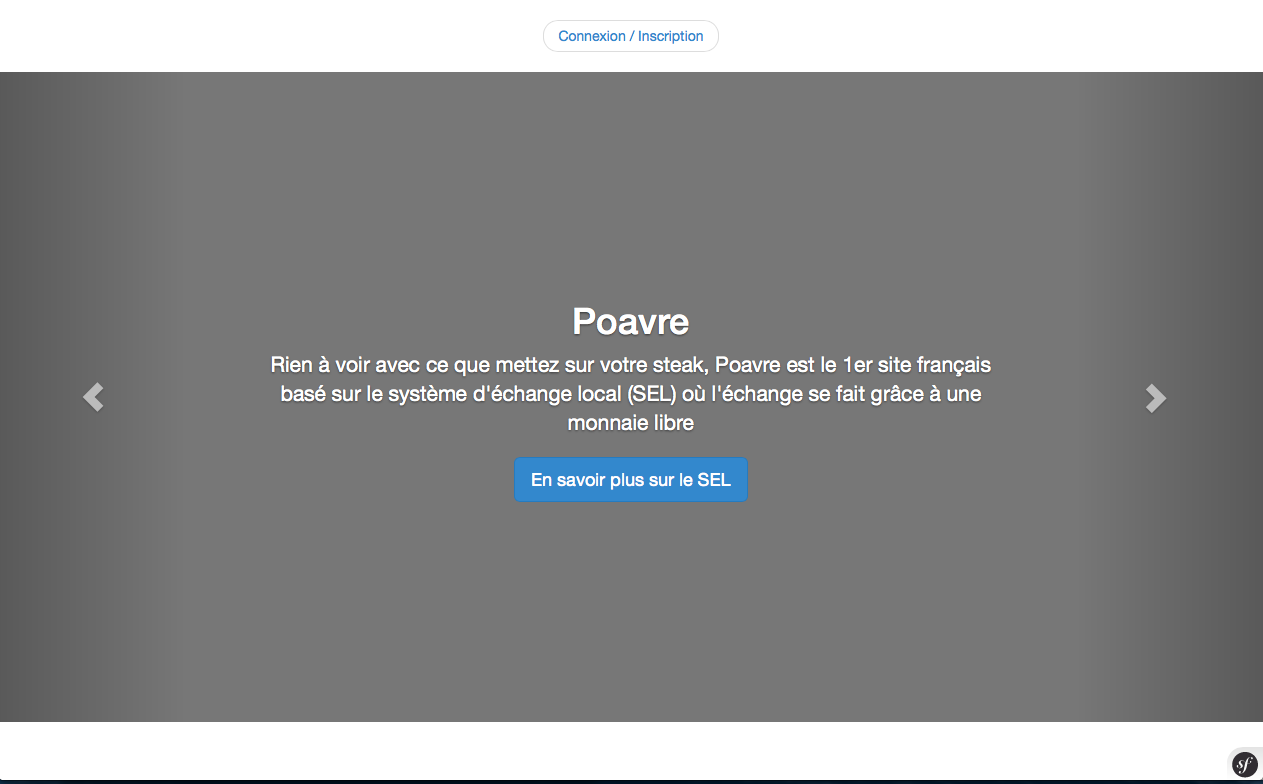
\includegraphics[width=1.0\textwidth]{cap1}
\caption{Page d'accueil du site}
\label{fig:accueil_site}
\end{figure}

%rajouter partie headerbar

\subsection{Choix du langage}
% auteur : Fabien
% relu par : Clément, Florian, Thin

Le choix du langage ou plutôt des langages est apparu naturellement lors de la présentation des différents outils de programmation.

Le PHP est indispensable ainsi que le CSS pour la mise en forme.

Quant au HTML, il sera utilisé au sein des templates Twig ce qui modifie légèrement la syntaxe car Twig ajoute des outils intéressants au niveau des vues.

Du JavaScript et du JQuery semblent utiles pour donner de la vie au site, notamment pour réaliser une page d'accueil dynamique, réactive et attrayante et pour la gestion des droits au sein des groupes ou du site d'une façon plus générale.

Au niveau de la langue, nous avions décidés initialement de réaliser un site cent pour cent anglophone (programmation, commentaires et affichage en anglais), puis finalement, après modification du code réalisé, nous sommes venus à une programmation en anglais, des commentaires en anglais mais un affichage en français car les utilisateurs finaux sont français.

\subsection{Choix du framework}
% auteur : Fabien
% relu par : Clément, Florian, Thin

Tout d'abord, nous avons établis qu'un framework serait plus judicieux pour la réalisation de ce projet c'est pourquoi les CMS présentés n'ont pas été retenus.

Aussi, nous voulions un framework puissant, mettant à notre disposition des fonctions utilisables pour notre projet afin de nous faciliter la programmation. Nous recherchions également un framework que nous pourrions utiliser à court terme, dans notre vie professionnelle.

CakePHP étant peu utilisé dans les entreprises françaises il n'a pas retenu notre attention. Il en va de même pour FuelPHP qui n'est quasiment pas utilisé en France. Finalement et avec enthousiasme Symfony2 a été choisi à l'unanimité pour ses performances, ses tutoriels mis à disposition (voir \cite{tuto_symfony}) et par sa forte utilisation au sein des entreprises françaises.

\subsection{Choix du serveur}
% auteur : Fabien
% relu par : Adrien, Clément, Florian, Thin

Au niveau de l'hébergement du site web il nous fallait un hébergeur acceptant une version récente de PHP, qui intégrait facilement des projets Symfony2 et qui donnait les pleins pouvoirs sur le projet de l'extérieur.

Nous avons tout d'abord pensé que nous pourrions héberger le site sur le serveur possédé par notre tuteur mais ce dernier ne s'est pas révélé compatible avec notre projet. Aussi, l'un des membres du projet ayant réalisé un projet avec Symfony2 antérieurement, nous avons décidé d'héberger notre site sur le même serveur à savoir celui de l'hébergeur Hostinger (voir \cite{hostinger}).

Ainsi, nous disposons d'un accès FTP (File Transfert Protocol) pour le transfert des fichiers vers le serveur, d'un accès à PHPMyAdmin qui stocke la base de données, d'une adresse mail propre au projet associée à l'hébergeur et de divers outils pratiques mais pas toujours utiles.

Ce serveur n'est pas dédié pour des raisons pécuniaires, il est donc partagé, mais les performances sont tout de même très bonnes et le site est accessible en tout temps.

\subsection{Choix du gestionnaire de projet et du gestionnaire 
de versions}
% auteur : Fabien/Adrien
% relu par : Clément, Quentin, Thin

\subsubsection{Le gestionnaire de projet}

Un outil de gestion de projet s'est révélé indispensable pour une réalisation efficace de ce projet. Il semblait important que celui-ci permette de gérer les différentes tâches de façon lisible et ordonnée.

Notre tuteur nous a présenté Producteev (voir figure \ref{fig:ScreenProducteev}), un outil de gestion de tâches en ligne et gratuit nous permettant de créer des tâches en spécifiant les collaborateurs leurs étant assignés ainsi que des «~suiveurs~» , afin que ces derniers soient informés par mail de leur avancée. Une échéance et une priorité peuvent être apposées sur les tâches et des sous-tâches qui peuvent également être commentés.

\begin{figure}[ht]
\centering
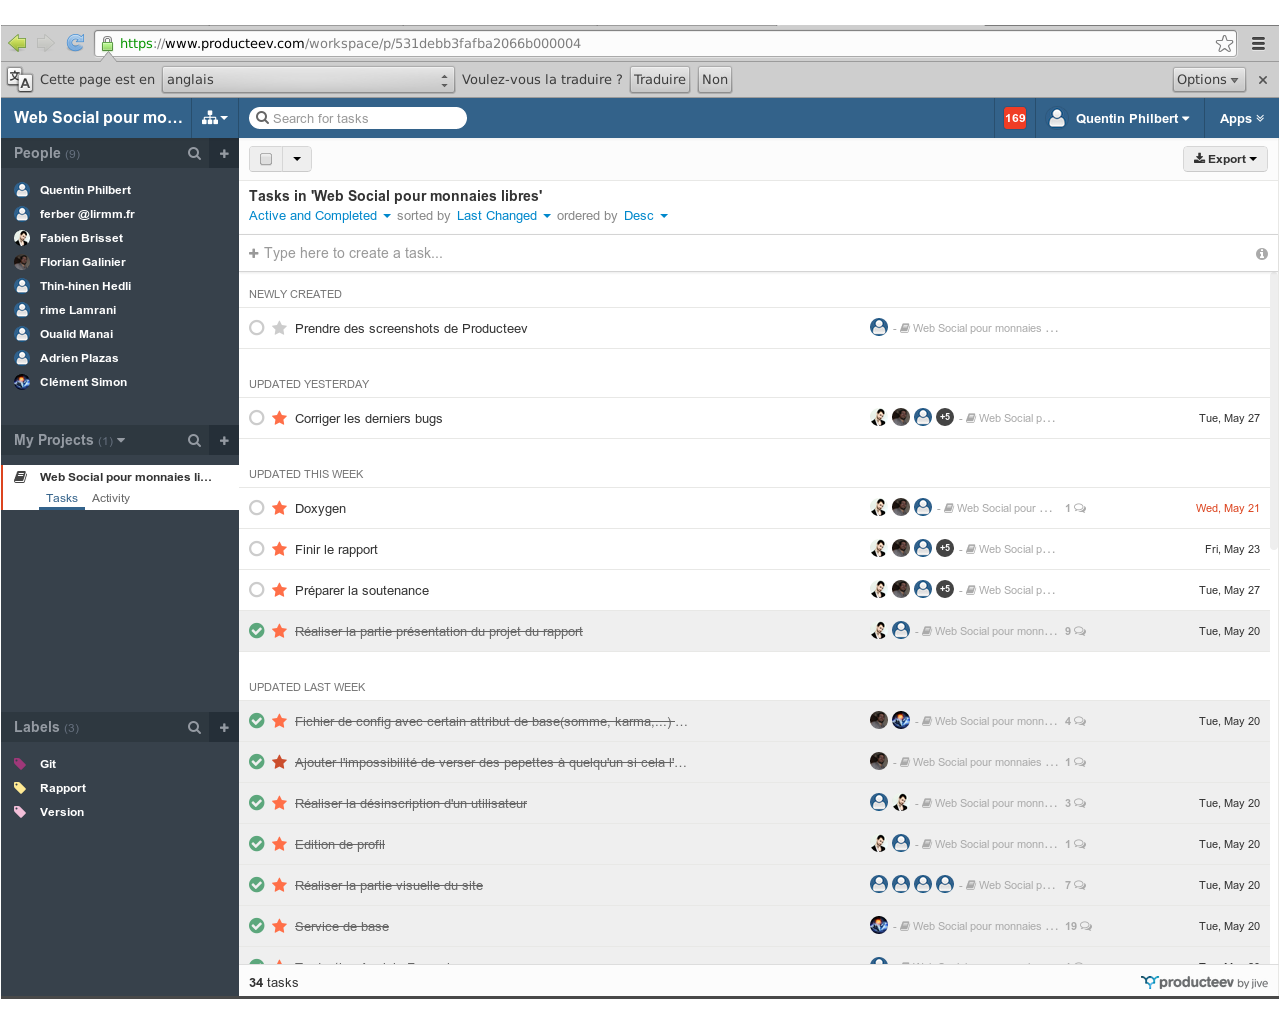
\includegraphics[width=0.9\textwidth]{ScreenProducteev}
\caption{Capture d'écran de Producteev}
\label{fig:ScreenProducteev}
\end{figure}

Le nombre de collaborateurs sur ce gestionnaire de tâche étant illimité, cet outil avec ses fonctionnalités est celui que nous avons choisi pour ce projet. En effet, nous ne nécessitions pas plus de fonctionnalités que celles-ci, nous n'avons donc pas cherchés d'autres outils pour la gestion des tâches du projet.

\subsubsection{Le gestionnaire de versions}

Un gestionnaire de versions semblait nécessaire afin de collaborer efficacement. Le gestionnaire de version distribué Git a rapidement été proposé, en association à Github (voir \cite{github}) pour l'hébergement du code du projet (voir \cite{progit}).
Après analyse des avantages et inconvénients par rapport à un système de gestion de versions centralisé comme SVN, notamment sur l'utilisation des branches, Git et Github ont été retenus.

\begin{figure}[ht]
\centering
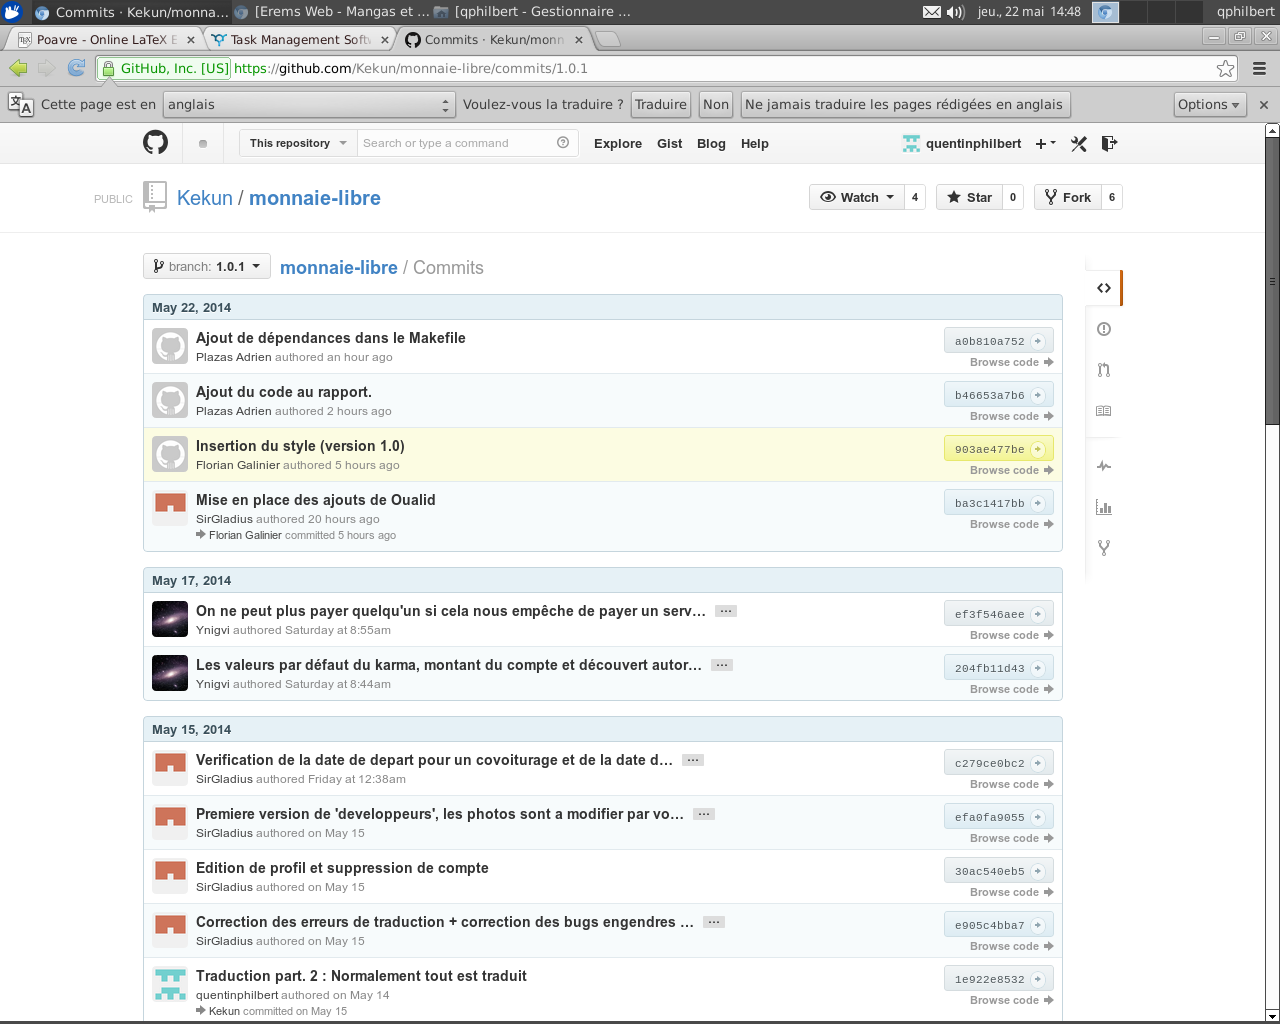
\includegraphics[width=0.9\textwidth]{ScreenshotGITHUB}
\caption{Capture d'écran de GitHub}
\label{fig:ScreenGitHub}
\end{figure}

\paragraph{Avantages}
Git est un gestionnaire de version très utilisé et il est apprécié pour sa robustesse, ses performances, sa praticité et sa capacité de mise à l'échelle (Git gère les versions du noyau Linux, une énorme base de code avec des milliers de collaborateurs).
De plus, cet outil est utilisable en lignes de commande sur de très nombreux systèmes d'exploitation (de Windows à Haiku en passant par Android).

\paragraph{Inconvénients}
Il demande à l'équipe d'apprendre de nombreux nouveaux concepts et son utilisation sur Windows peut être laborieuse, de par son interface en ligne de commande.

\subsection{Choix des outils de documentation}
% auteur : Adrien
% relu par : Fabien, Clément, Thin

Doxygen (voir \cite{doxygen}) est apparu comme un choix évident pour la documentation~:
\begin{itemize}
    \item c'est un logiciel libre, solide et puissant~;
    \item il n'est pas spécifique à un langage et fonctionne bien avec PHP~;
    \item il est assez simple à appréhender~;
    \item sa syntaxe est simple et lisible telle quelle comme documentation dans le code, le rendant assez peu intrusif.
\end{itemize}
Il répond parfaitement à nos besoins de documentation et il n'est pas étonnant qu'il soit devenu un leader dans son domaine.


\chapter{Analyse}

\section{Analyse des besoins}
% auteur : Rime
% relu : Fabien, Clément, Florian, Quentin

L’objectif initial était de réaliser un site communautaire, permettant à ses utilisateurs de proposer des services entre eux par l’échange d'une monnaie libre a travers un site épuré et agréable. 
Il a été nécessaire que l’on se réunisse plusieurs fois, afin de donner forme a ce projet, d’en dessiner les contours, de définir les tenants et les aboutissants. 
En effet, il était primordial de savoir exactement ce que ce site doit apporter. En quoi est-il intéressant~? A qui s’adresse-t-il en particulier~? Que propose-t-il de plus ou de différent par rapport aux sites existants~? Pourquoi, in fine, l’utilisation d’une monnaie libre~? 

Ce n’est que par cette analyse préalable, que nous avons pu identifier correctement les tâches à réaliser, les limites de notre projet et les éventuelles améliorations futures, dans une perspective d’évolution.

La première étape, s’est portée plus sur le fond que sur la forme ou la technicité. Il s’agissait de se donner un maximum d’idées sur ce que le site devait proposer. 
Vis à vis de l’objectif initial, il paraissait important de spécifier au mieux les services auxquels se rattache notre projet. C’est à dire, ce qu’il permettait de faire pour ses utilisateurs. Pour nous il était intéressant qu’un utilisateur puisse à la fois bénéficier de services et/ou en proposer. L’utilisateur de notre site devait donc avoir la possibilité, à sa guise, d’être un producteur et/ou un consommateur de services. Il devait être maître, non seulement, du choix du service qu’il désire (évident) mais aussi du type et de la hauteur de sa rétribution pour le service qu’il proposerait. 

Il apparu assez évident que les types d’échanges se porteraient essentiellement sur des services à la personne, d’aide et de partage (type covoiturage, couchsurfing et troc). 
À priori, un site comme le Bon coin (voir \cite{bc}) le permettait déjà. Cependant, c’est là que l’idée de monnaie libre nous distinguait de l’existant. Jusqu’à présent, le principal modèle de rétribution d’un service était celui de l’argent. À ce modèle encore largement prédominant, apparaissait de plus en plus des réponses de substitution. La monnaie libre permettrait de générer des échanges de services entre individus sans argent réel. Ce projet s’inscrit donc dans une perspective d’utilité sociale par la proposition d’un modèle alternatif d’échange de services. 

\section{Analyse de l'existant}
% auteur : Fabien
% relu : Clément, Florian

Des SELs (Système d'Echange Local) existent dans plusieurs régions de France sous forme de «~réunions~» où les différents usagers peuvent communiquer et échanger leurs services. 
Ce type d'échanges ne semble pas au goût du jour, en effet, l'Informatique a pris une place prépondérante dans notre système, dans notre mode de vie.
L'idée de proposer ces échanges par le biais de l'outil informatique est donc d'un enjeu important car elle en permet une adaptation moderne et pratique.
Un SEL en ligne existait déjà, «~Flowplace~» (voir figure \ref{fig:flowplace}), mais il ne semblait pas tout à fait effectif, il a, semble-t-il, d'ailleurs fermé à ce jour.
Nous étions donc libre d'imaginer comme nous le souhaitions notre site.

\begin{figure}[ht]
\centering
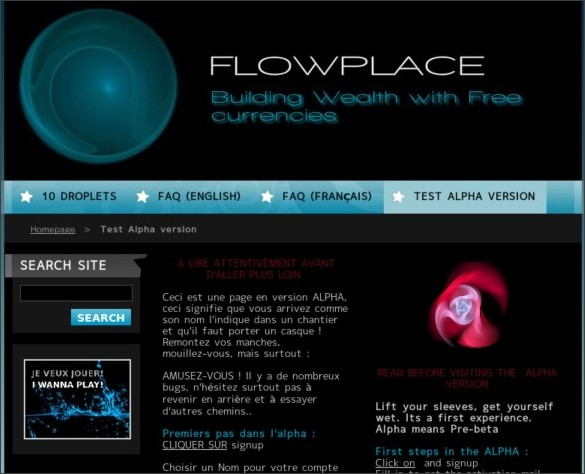
\includegraphics[width=0.9\textwidth]{flowplace}
\caption{Flowplace}
\label{fig:flowplace}
\end{figure}

\subsection{Analyse préalable}
% auteur : Rime
% relu par : Fabien, Clément, Florian

Lors de l'analyse, le référentiel utilisé fut le point de vue de l’utilisateur de notre site. 
Il fut décidé d'identifier un utilisateur par son nom, son prénom et son pseudo.
Il fut également choisi d'attribué à l'utilisateur une grandeur quantifiable nommée Karma, en référence à l’ensemble des bonnes et mauvaise actions qu’il aura réalisé au cours de son activité sur le site. Cette grandeur peut s'apparenter à une note de satisfaction, attribuée par les autres utilisateurs auxquels il aurait rendu service.
L'idée de proposer des «~missions~» aux utilisateurs fut aussi abordée, mais ne fut finalement pas retenue pour le projet final. Ces «~missions~» devaient être un ensemble des services qu'un utilisateur devait effectuer ou proposer, recevant en échange des récompenses monétaires et/ou en karma.
Nous abordions également le thème de la «~monnaie~». Un utilisateur devait pouvoir choisir de «~payer~» ou de se faire «~payer~» dans la monnaie libre du site, complètement décorrélée de quelconque monnaie existante. Cela devait s'apparenter à une quantité de «~points~» qui permettrait l’échange de prestations entre utilisateurs. 

Au départ, un nouvel utilisateur devait posséder un Karma neutre et une quantité de monnaie qui pourraient fluctuer au cours de son activité intra-site.

Chaque utilisateur devait également être attaché à un compte unique. Ce compte enregistrerait les diverses transactions et calculerait dynamiquement le solde restant, à l'instar d'un compte bancaire.

L'idée de groupe fut également abordé. Chaque membre pouvaient faire partie d'un ou plusieurs groupes. 
À ces groupes devait également être rattachée une liste de services.

\section{Diagrammes de cas d'utilisation}
% auteur : Quentin
% relu : Clément

\subsection{Cas d'utilisation : Membre}

\begin{figure}[ht]
\centering
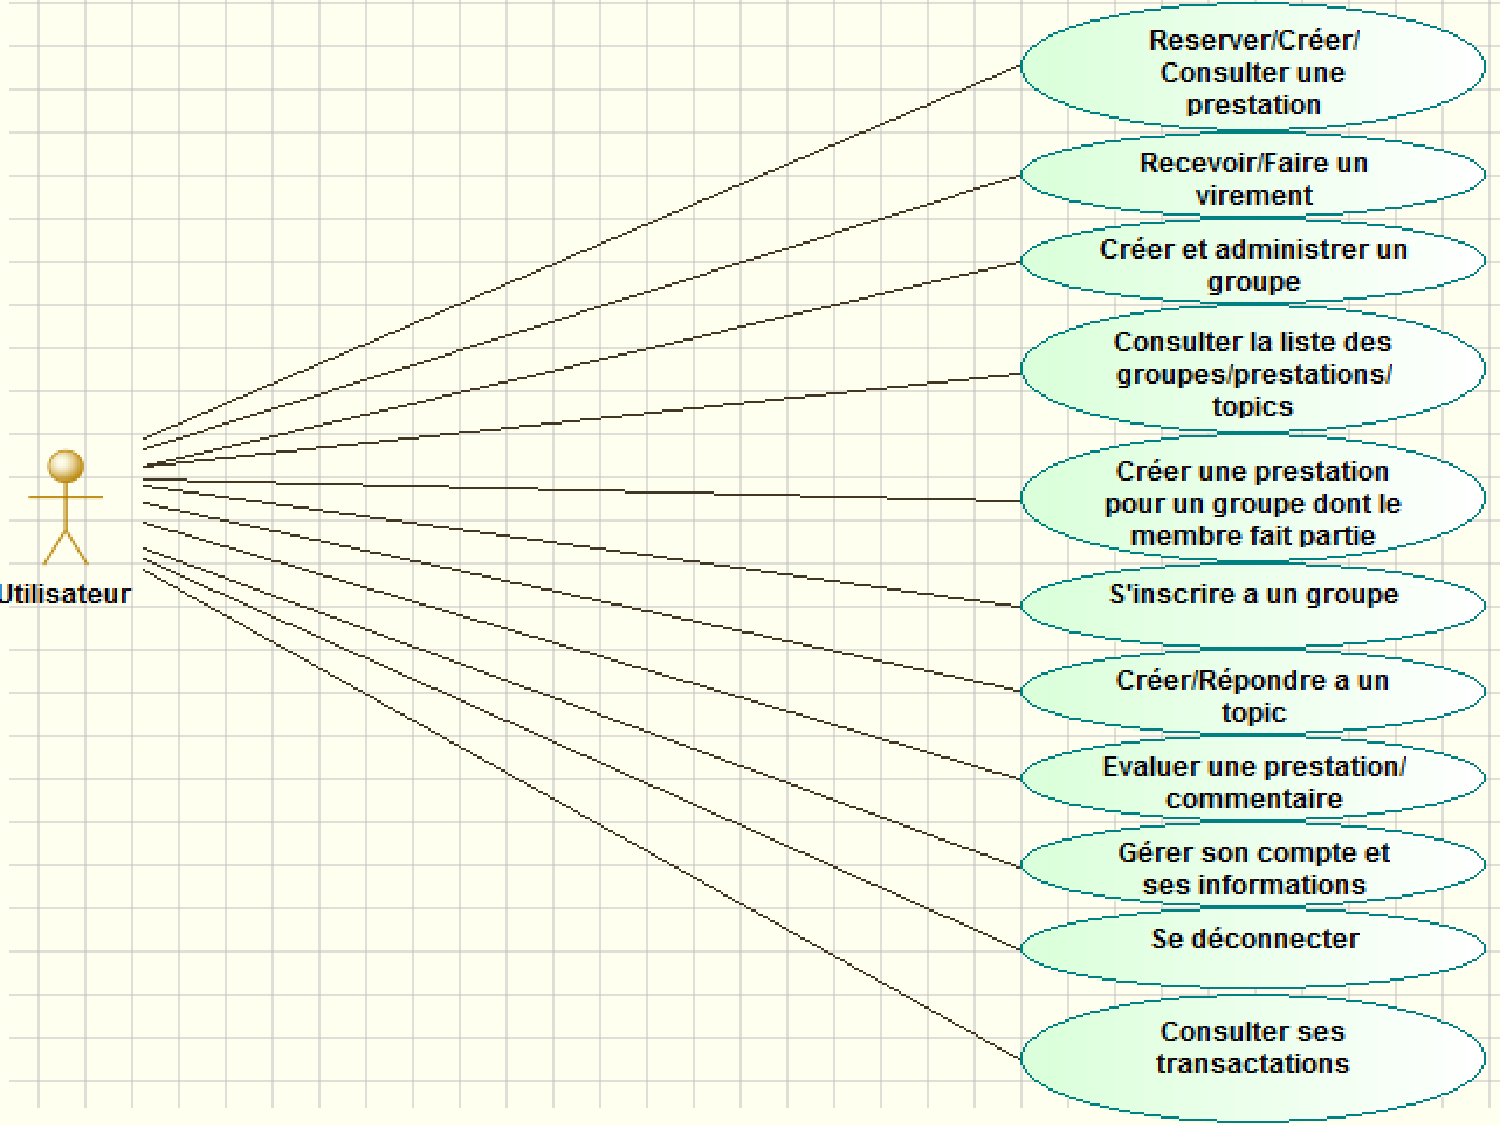
\includegraphics[width=0.9\textwidth]{UseCaseUtilisateur}
\caption{Diagramme de cas d'utilisation d'un utilisateur}
\label{fig:UseCaseUtilisateur}
\end{figure}

A la figure \ref{fig:UseCaseUtilisateur} nous pouvons constater les actions qui sont disponibles pour un membre.
Un membre peut donc réserver, créer ou consulter une prestation, faire ou recevoir un virement, créer et administrer un groupe de membres, consulter la liste des groupes, prestations et topics, créer une prestation pour un groupe dont le membre fait partie, s'inscrire à un groupe, créer et répondre à un topic, évaluer un topic ou une prestation, gérer son compte et ses informations et, enfin, se déconnecter.

\subsection{Cas d'utilisation : Modérateur}

\begin{figure}[h]
\centering
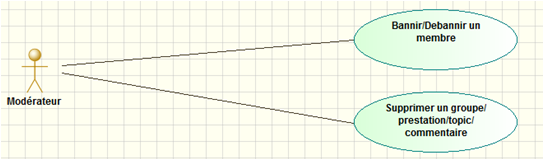
\includegraphics[width=0.9\textwidth]{UseCaseModerateur}
\caption{Diagramme de cas d'utilisation d'un modérateur}
\label{fig:UseCaseModerateur}
\end{figure}

A la figure \ref{fig:UseCaseModerateur} nous pouvons constater les actions qui sont disponibles pour un modérateur.
Un modérateur a pour responsabilité de veiller à ce que les services soient corrects, qu'il n'y ait pas d'abus au niveau des interactions entre les utilisateurs.
Pour mener cette tâche à bien, un modérateur peut bannir ou débannir un membre, supprimer un groupe, une prestation ou encore un topic.

\section{Diagrammes de classes}

\subsection{Diagramme de classe prévisionnel}
% auteur : Oualid, Quentin
% relu par : Clément, Florian

\begin{figure}[ht]
\centering
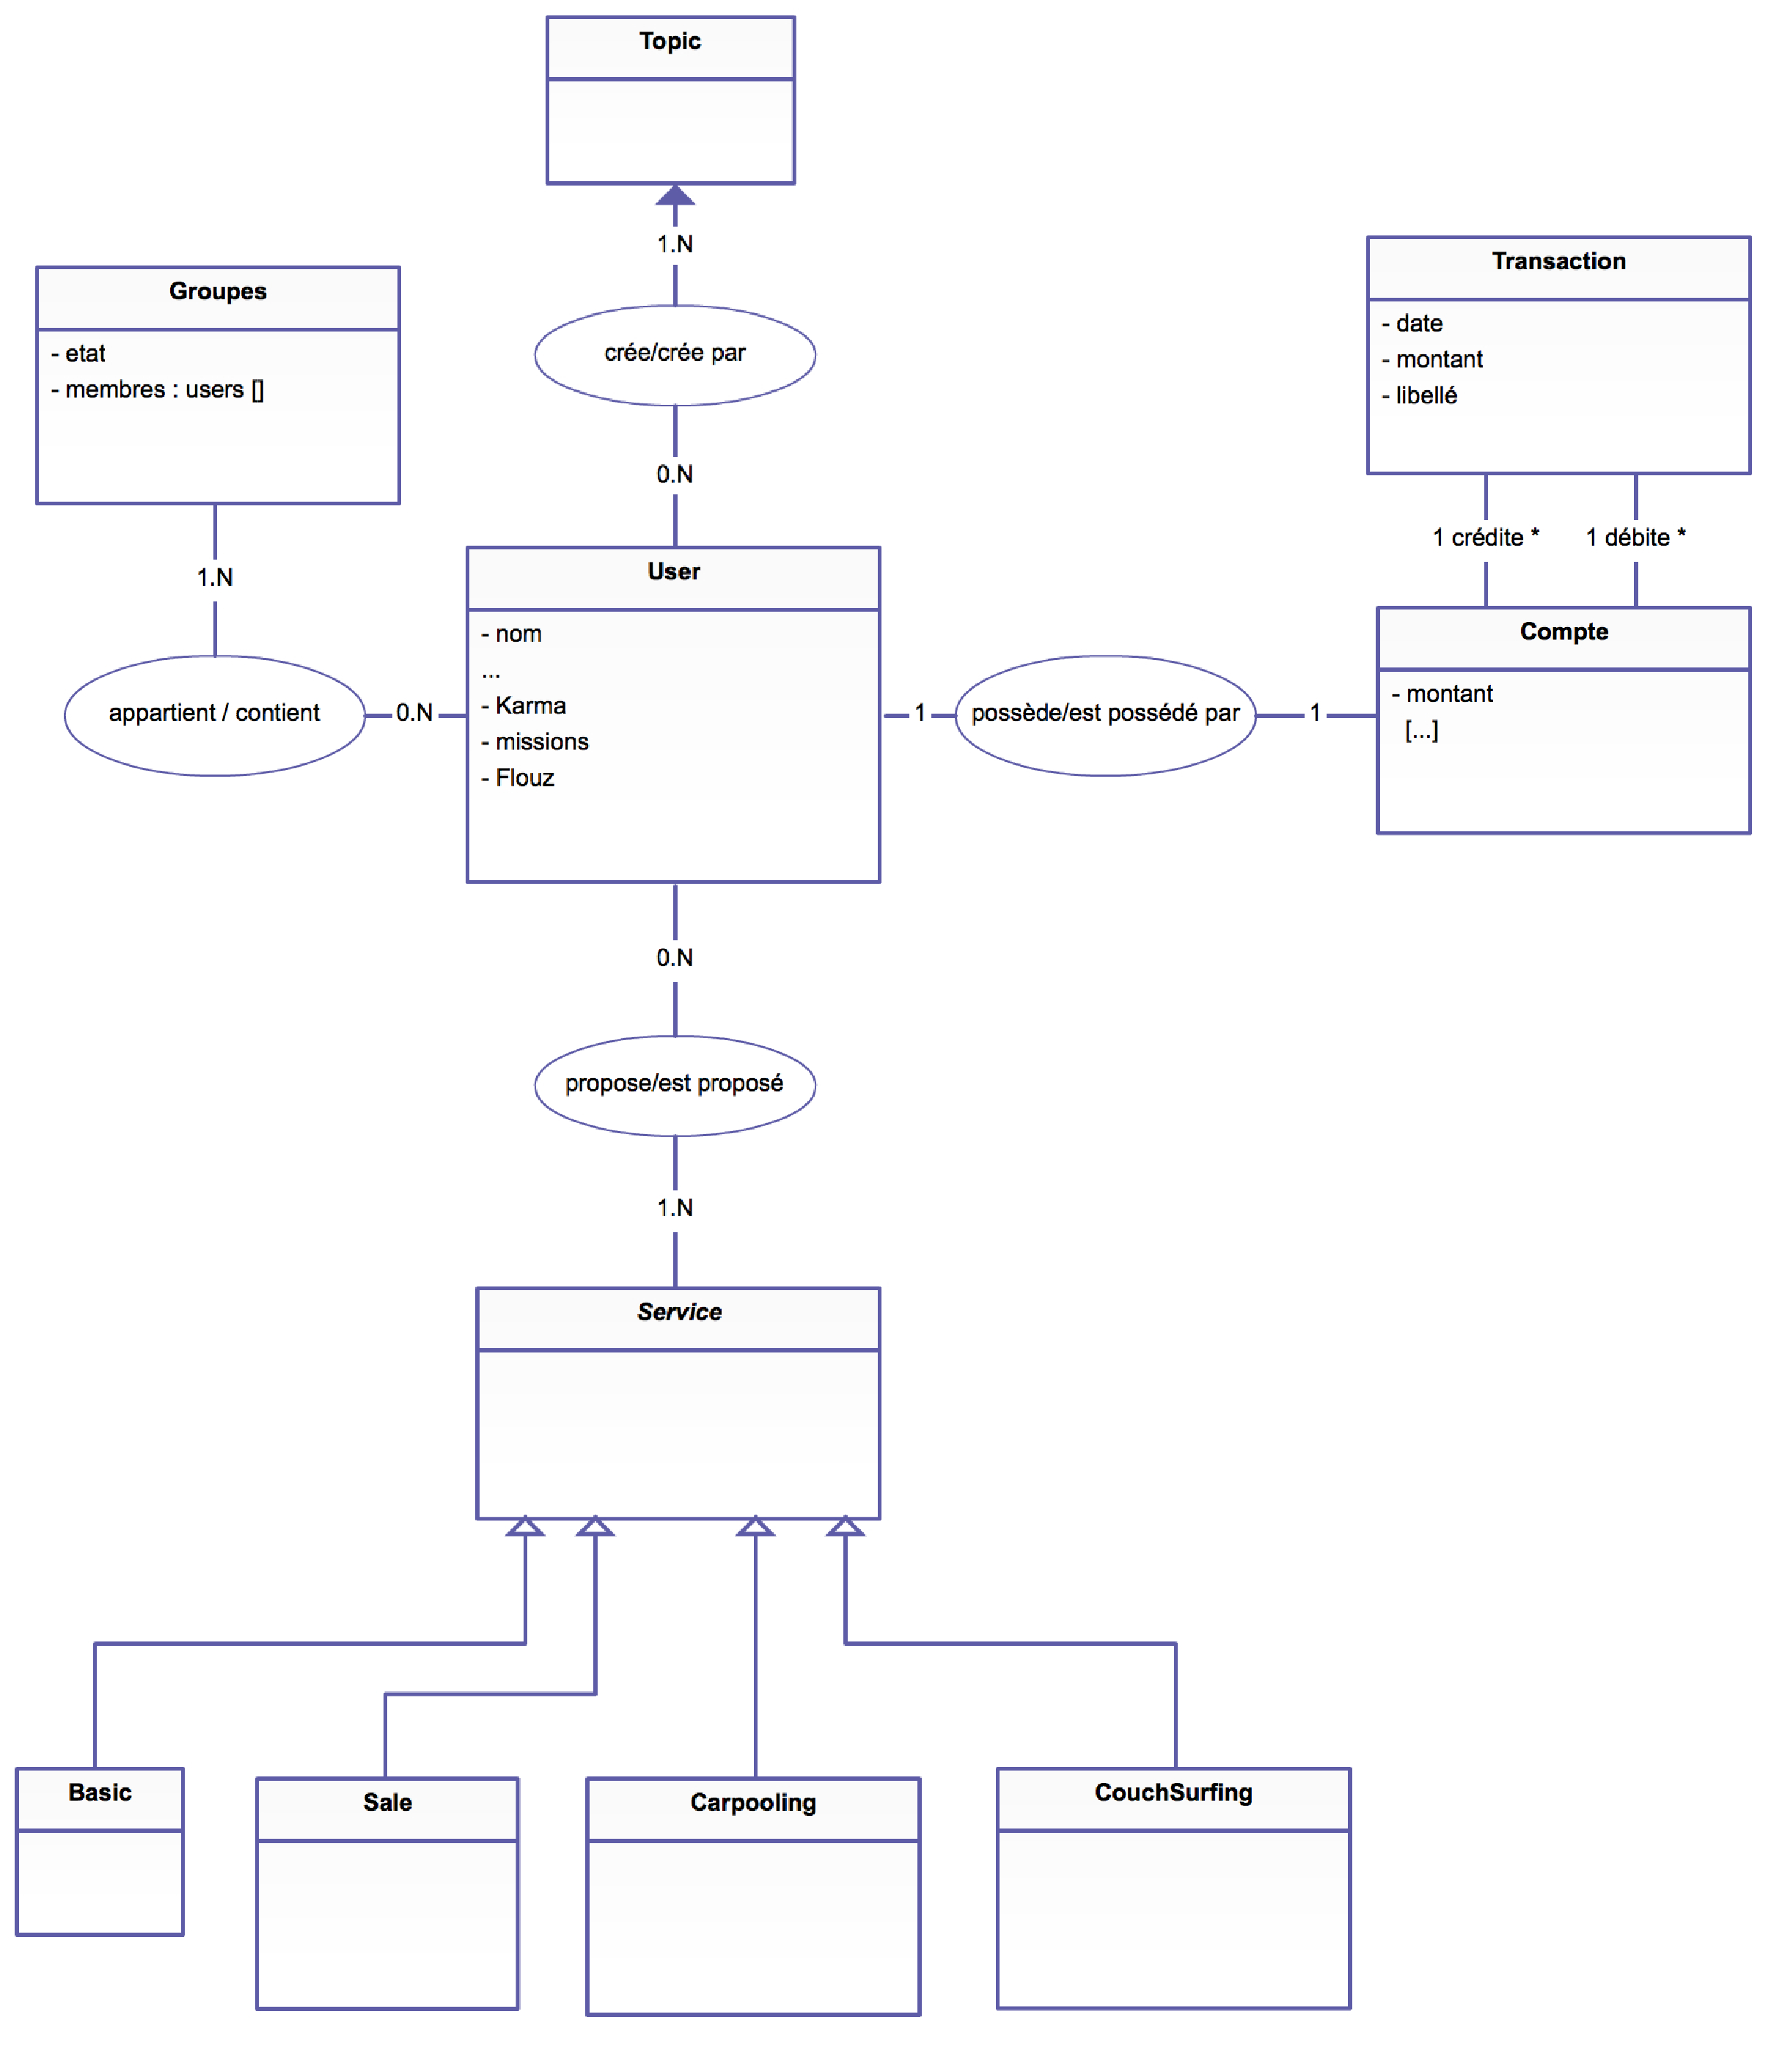
\includegraphics[width=0.9\textwidth]{diagramme-classe-previsionnel2}
\caption{Diagramme de classe prévisionnel}
\label{fig:diagramme-classe-previsionnel2}
\end{figure}

La figure \ref{fig:diagramme-classe-previsionnel2} représente la modélisation du système au niveau des classes que nous avions prévues avant de commencer à coder. 
Il a ensuite bien évolué...

\subsection{Diagramme de classe final}
% auteur : Oualid, Quentin
% relu par : Florian, Clément
\begin{figure}[ht]
\centering
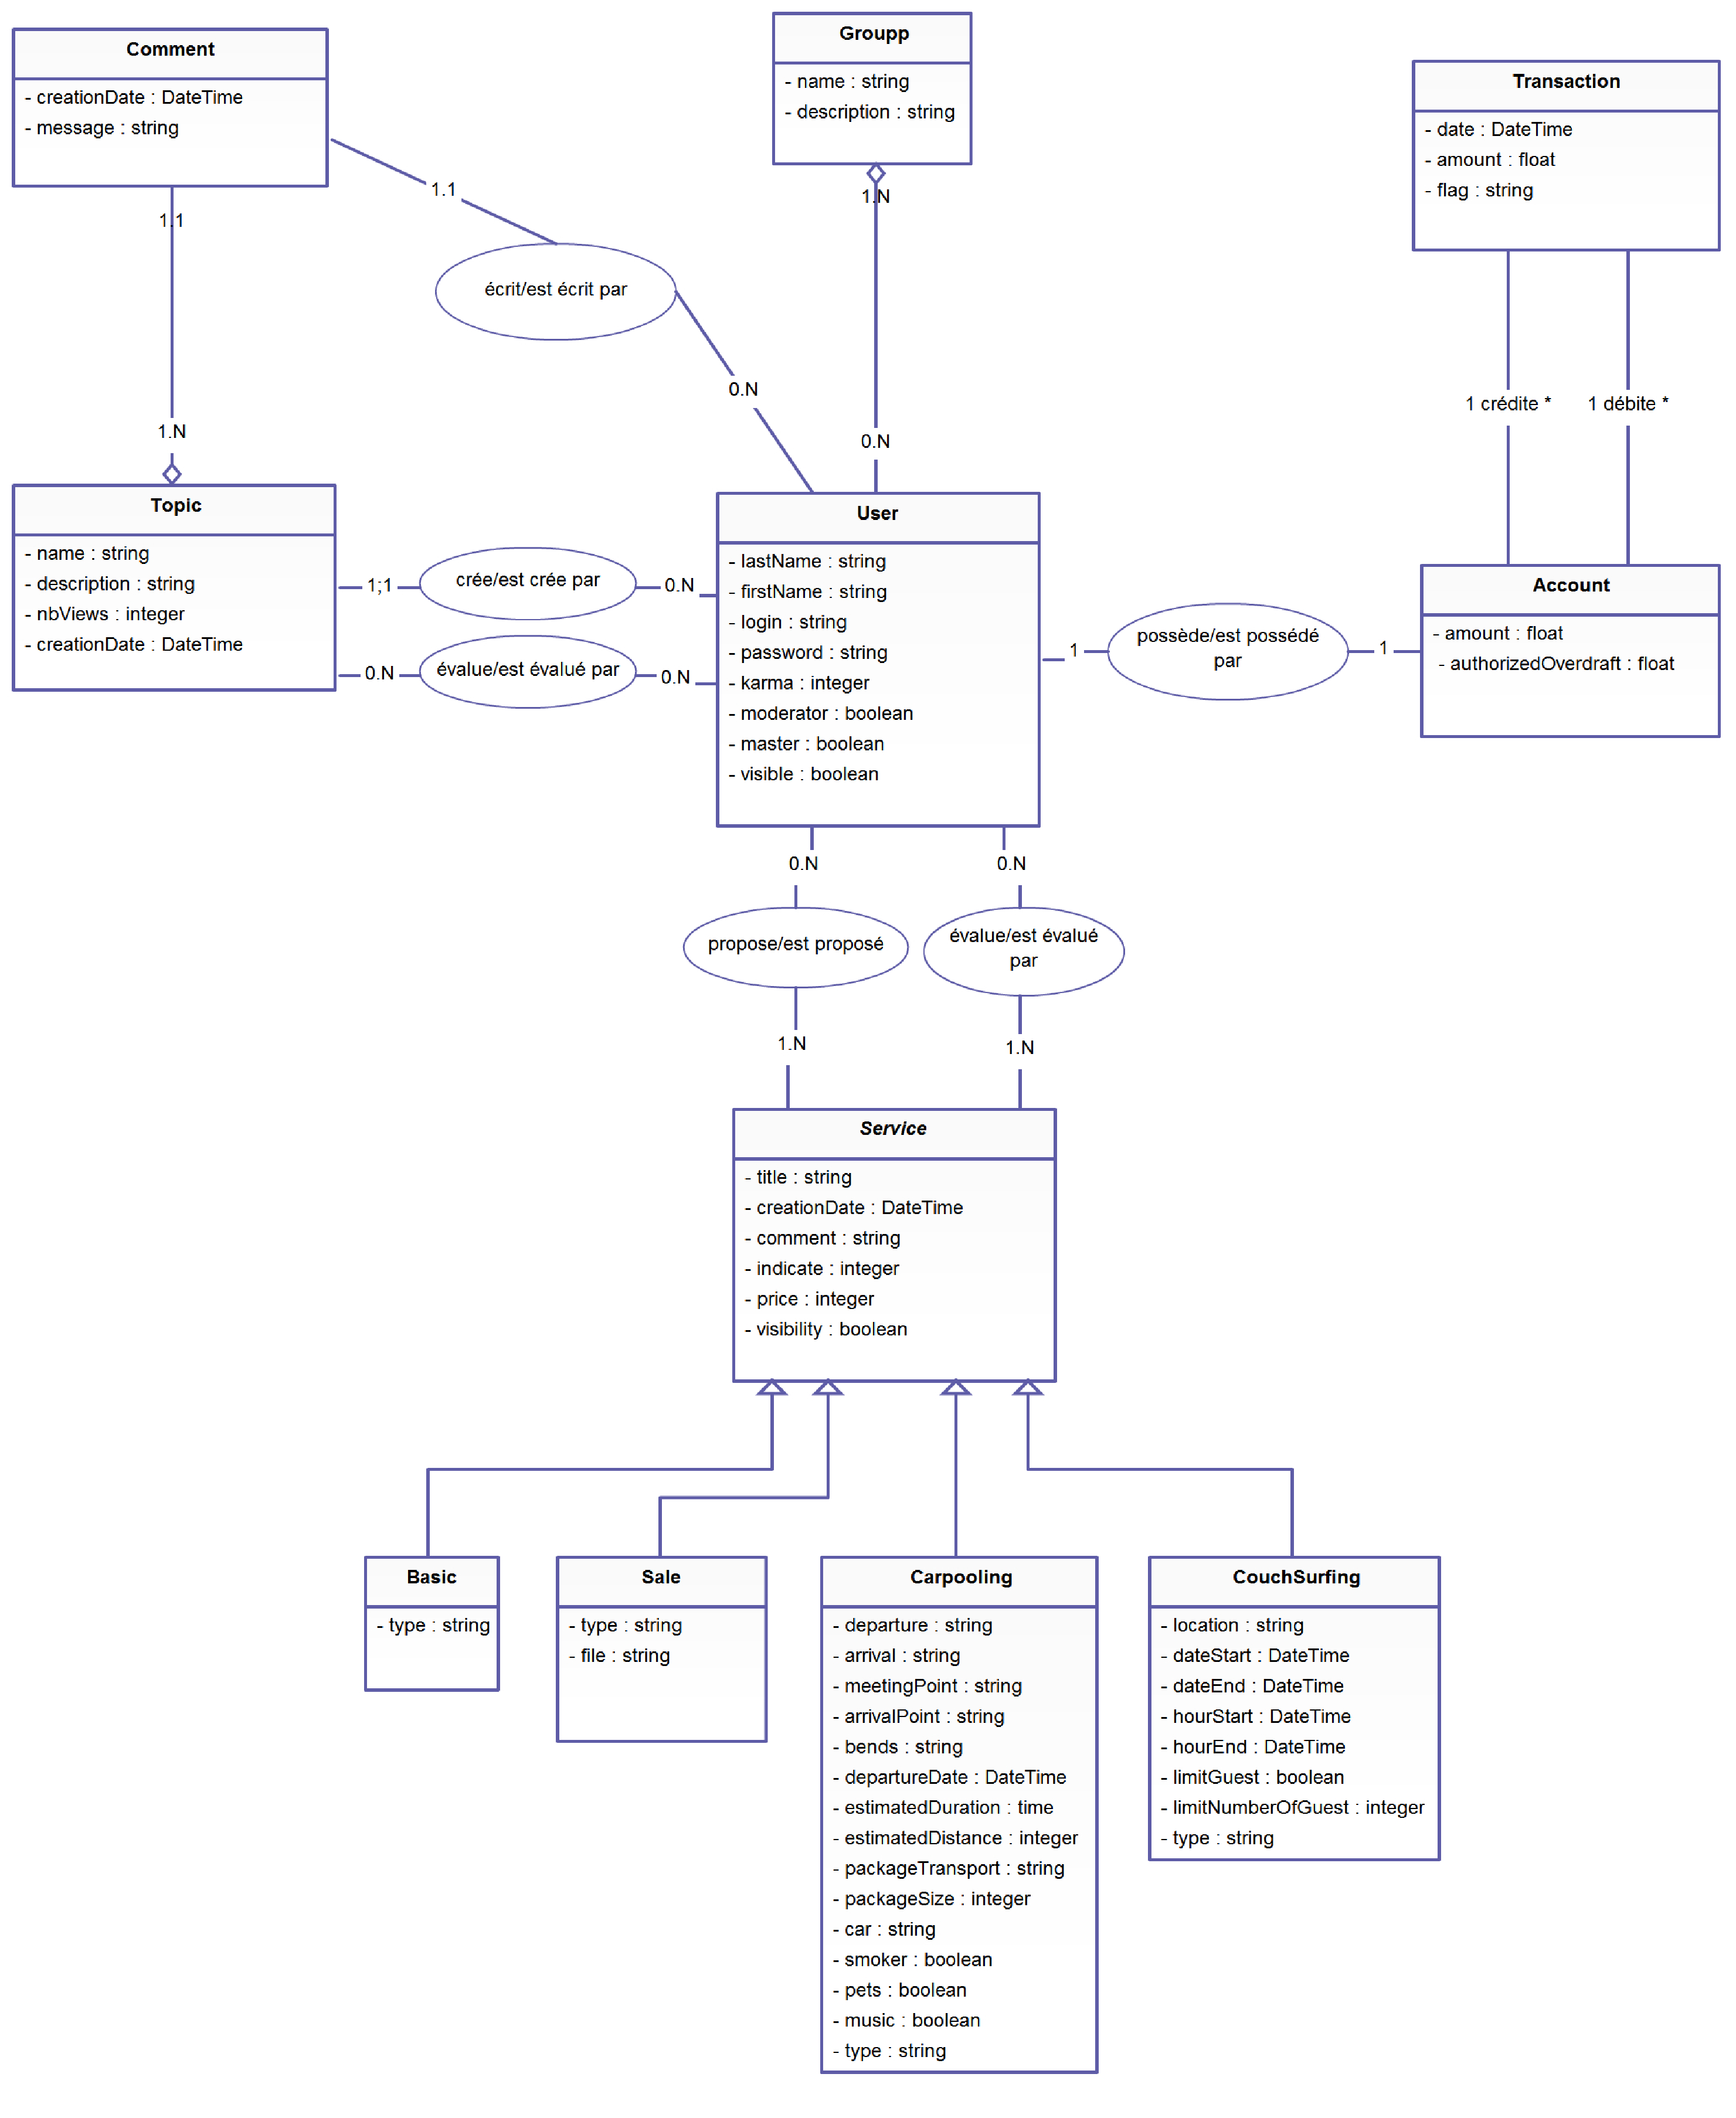
\includegraphics[width=1.0\textwidth]{diagramme-classe-final}
\caption{Diagramme de classe final}
\label{fig:diagramme-classe-final}
\end{figure}

Le diagramme qui apparaît à la figure \ref{fig:diagramme-classe-final} représente nos classes d'un point de vue conceptuel. C'est le diagramme de classe final, il implémente actuellement notre système.

% auteur : Rime
% relu : Fabien, Florian, Clément

Notre diagramme prévisionnel a évolué vers son état final en ce diagramme. 
Cette fois-ci les services se divisent en quatre grandes catégories :
\begin{description}
\item [Couchsurfing] qui correspond à trouver/proposer un logement temporaire~;
\item [Covoiturage] qui permet un déplacement à plusieurs partageant ainsi les coûts inhérents au voyage~; 
\item [Ventes] qui, à l’instar de sites comme Le Bon Coin ou encore Ebay, permet des échanges d'objets~; 
\item [Basique] qui correspond à tout ce qui est autre que les trois catégories pré-citées.
\end{description}

La possibilité pour chaque utilisateur d’utiliser un forum afin de favoriser le lien social et d’expliciter éventuellement au mieux sa demande et/ou proposition. 
Le karma quant à lui est toujours une quantité qui fluctue en fonction des évaluations des autres utilisateurs ayant bénéficiés du service fourni. 
De plus, chaque classe a été définie par un certain nombre d’attributs qui sont plus précis que ceux du diagramme prévisionnel. Ceux-ci sont commentés plus spécifiquement dans la section en rapport avec les bundles.



%%%
%%% Ce chapitre est terminé, il a été intégré au rapport.
%%% Toute modification ultérieure devra être signalée à Adrien qui s'occupe de son intégration.
%%%

\chapter{Réalisation du projet}

\section{Les bundles}
% auteur : Clément
% relu par : Fabien, Adrien, Oualid

Afin de réaliser le projet, nous avons décidé de découper le travail en bundles s'occupant chacun d'une partie précise du site, afin de simplifier la naviguation entre ces parties.
Chaque bundle gère une partie du modèle, de la vue et du contrôleur de l'application. Un bundle possède son propre nom de la manière suivante, suffixé par \verb|Bundle| (par exemple, le bundle \verb|User| est nommé \verb|UserBundle|).

Le modèle est géré dans le dossier \verb|Entity|, où toutes les classes seront implémentées.

Le contrôleur se trouve dans le dossier \verb|Controller|, un contrôleur effectue des contrôles sur le modèle avant d'envoyer les données à la partie vue.
Dans Symfony, les opérations d'un contrôleur sont sous forme de méthodes suffixées par \verb|Action|.

Les vues sont répertoriées dans le dossier \verb|Ressources/views|, on y retrouve donc les différentes vues en lien avec le contrôleur et les modèles donnés.

% Ici Adrien :
% Je vous propose d'expliquer ce que fais spécifiquement chaque bundle dans la partie bundle sans rentrer dans le détail de comment fonctionne un bundle de manière globale pour le faire dans les trois sections suivantes (M, V et C)
% Ainsi on pourra expliquer ce que font les bundles (exemple: se connecter, échanger de l'argent...) plutôt que comment ils fonctionnent

\subsection{Le bundle User}
% auteur : Clément
% relu par : Florian, Fabien, Adrien, Oualid

Le bundle \verb|UserBundle| implémente l'entité utilisateur qui comporte les attributs types d'un utilisateur~: pseudo, mot de passe (encodé en MD5), nom, prénom, date de naissance, karma, ...

Le contrôleur permet d'effectuer différentes opérations liées à un utilisateur. En voici les différentes fonctionnalités~:
\begin{description}
    \item [indexAction] si un utilisateur vient de se connecter la méthode \verb|seeAction| est appelée, sinon la page d'inscription/connexion est affichée~;
    \item [seeAction] affiche le profil d'un utilisateur~;
    \item [addAction] vérifie si les données d'inscription ne sont pas redondantes avec des données déjà contenues dans la base de données~: si elles ne le sont pas un nouvel utilisateur est créé et la méthode \verb|seeAction| est appelée, sinon le formulaire est généré à nouveau dans le but d'être rempli correctement~;
    \item [deleteAction] supprime l'utilisateur et tous les services qui y sont associés~;
    \item [connectionAction] connecte un utilisateur en fonction de son login et de son mot de passe~;
    \item [deconnectionAction] déconnecte un utilisateur du site et le redirige vers la page de connexion~;
    \item [editAction] un utilisateur, une fois connecté, peut modifier son profil.
\end{description}

\subsection{Le bundle Service}
% auteur : Clément
% relu par : Fabien, Adrien, Oualid

Ce bundle catégorise les différents types de service existants sur le site, implémentés par des entités séparées, que sont~: service de base, covoiturage, vente et couchsurfing.

Chaque service contient~:
\begin{itemize}
    \item un identificateur~;
    \item un titre~;
    \item une date de création~;
    \item une description~;
    \item un prix~;
    \item une visibilité~;
    \item un groupe associé (ou non)~;
    \item une liaison avec un utilisateur à travers l'entité \verb|ServiceUser| et ses dérivés~;
    \item un type de service qui permet de définir s'il s'agit d'un service de base, d'une vente, d'un covoiturage ou d'un couchsurfing.
\end{itemize}

Le contrôleur quant à lui, fonctionne via les méthodes suivantes~:
\begin{description}
    \item [indexAction] énumère tous les services existants selon un type de classement choisi (par date de création par défaut, par créateur, par type de service, par prix croissant ou décroissant)~;
    \item [addServiceAction] appelle la méthode de création du service que l'on veut créer~;
    \item [seeBasicAction et ses dérivés] permet de voir son service~;
    \item [addBasicAction et ses dérivés] permet d'ajouter son service, à un groupe si on le désire~;
    \item [deleteBasicAction et ses dérivés] permet de supprimer son service~;
    \item [seeMyServicesAction] répertorie tous les services que l'on propose, qu'ils soient réservés ou non~;
    \item [serviceDoneAction] est appelé pour spécifier qu'un service a été effectué.
\end{description}

\subsection{Le bundle Transaction}
% auteur : Florian
% relu par : Clément, Fabien, Adrien, Oualid

Ce bundle avait pour objectif premier la gestion des comptes «~monétaires~» des utilisateurs. Par la suite, la partie évaluation s'est ajoutée à ce bundle, afin de faire le lien entre un service et un paiement.

Les différentes entitées de ce bundle sont~:
\begin{description}
    \item [Account] cette entité contient un identifiant de compte, un montant de compte ainsi qu'un découvert autorisé~;
    \item [Transaction] cette entité est chargée de stocker une transaction entre deux comptes, c'est à dire les deux comptes concernés, le montant de la transaction ainsi qu'un libellé optionnel~;
    \item [Evaluation et ses dérivés] cette entité fait le lien entre un service souscrit par un utilisateur ainsi qu'une note, précisant si le service a été payé ou non~; l'évaluation sera considérée comme «~à faire~» tant qu'elle n'aura pas été payée.
\end{description}

Il existe ainsi dans ce bundle deux contrôleurs~:
\begin{description}
    \item[TransactionController] ce contrôleur gère les actions effectuées entre deux comptes~:
    \begin{description}
        \item[indexAction] appelle la vue qui affiche, si l'utilisateur est connecté, la liste de ses transactions~;
        \item[paymentAction] appelle la vue qui affiche un formulaire permettant de faire un virement vers un autre utilisateur et traite le formulaire lors de la soumission~;
    \end{description}
    \item[EvaluationController] ce contrôleur gère l'évaluation et le paiement lorsqu'un service est effectué~:
    \begin{description}
        \item[indexAction] appelle la vue qui affiche, si l'utilisateur est connecté, la liste de tous les services en attente d'évaluation~;
        \item[evaluationAction] permet à l'utilisateur d'attribuer une note à un service effectué et de le payer, en gérant automatiquement la soumission du formulaire d'évaluation, effectuant le paiement et évaluant le karma (via la méthode \verb|evalKarma|)~;
        \item[evalKarma] qui va recalculer le karma attribuées à l'utilisateur passé en paramètre en faisant une moyenne arithmétique de toutes les notes ramenées sur 100 (les notes sont sur 10, le karma est sur 100).
    \end{description}
\end{description}

\subsection{Le bundle Group}
% auteur : Fabien
% relu par : Clément, Adrien, Oualid

Ce bundle est utilisé pour regrouper les utilisateurs autour de services.

\begin{description}
    \item [Groupp] est une entité qui permet le groupement d'utilisateurs par un identifiant unique, un nom et une description ainsi qu'un administrateur, cette entité se nomme \verb|Groupp| car \verb|Group| est un terme réservé par Symfony2~;
    \item [associatedGroup] est un attribut de l'entité \verb|Service| qui permet d'associer un service à un groupe~; ce service figurera dans la vue \verb|see_group.html.twig\verb| du groupe associé.
\end{description} 

\verb|GroupController| est le contrôleur qui permet de gérer les groupes, à savoir, les afficher, afficher un groupe en détails, ajouter un utilisateur, bannir un utilisateur, demander à rejoindre un groupe, supprimer une demande pour rejoindre un groupe et supprimer un groupe.

\subsection{Le bundle Forum}

% auteur : Fabien
% relu par : Clément, Adrien, Oualid

Ce bundle est utilisé pour la communication entre les membres de Poavre sur divers sujets, cela peut être de la communication pure (chat), de la communication sur les services proposés ou encore débattre sur des sujets et proposer des nouveautés à apporter au site.

\begin{description}
    \item [Topic] (ou sujet) est une entité qui possède un identifiant unique, un ratio d'approbation (likes/dislikes), un nom, une description, une date de création, un nombre de vues et un auteur~;
    \item [Comment] est une entité qui possède un identifiant unique, un message, une date de création et un auteur~;
    \item [TopicComment] est une entité associative (une association) entre les entités \verb|Topic| et \verb|Comment|, ainsi un commentaire est propre à un sujet qui dispose de plusieurs commentaires~;
    cette entité possède deux attributs, l'un référençant le sujet et l'autre référençant le commentaire~;
    \item [TopicUser] est une entité associative (une association) entre les entités \verb|Topic| et \verb|User|, ainsi, un utilisateur peut commenter plusieurs sujets et même plusieurs fois le même sujet et chaque sujet est commenté par plusieurs utilisateurs~ ;
    cette entité possède deux attributs, l'un référençant le sujet et l'autre référençant l'utilisateur.
\end{description} 

\verb|ForumController| est un contrôleur qui permet de gérer les sujets et commentaires, à savoir, afficher la liste des sujets, afficher, créer, commenter, «~liker~» et «~disliker~» un sujet.

\subsection{Le bundle Home}

% auteur : Fabien
% relu par : Clément, Adrien, OUalid

Ce bundle est utilisé pour l'affichage de la page d'accueil du site ainsi que pour l'accès à l'onglet «~Développeurs~».
Ainsi la majeure partie des redirections se font soit vers la création de compte utilisateur ou de connexion, soit vers la page d'accueil.

\verb|HomeController| est un contrôleur qui permet l'affichage de la page d'accueil du site ainsi que l'accès à l'onglet «~Développeurs~».

\subsection{Le bundle Administration}

% auteur : Fabien
% relu par : Clément, Adrien, Oualid

Ce bundle est utilisé pour la gestion de Poavre par les modérateurs du site.

\verb|AdministrationController| est un contrôleur qui permet à un administrateur de bannir des membres, les nommer modérateur ou «~master~» (utilisateur suprême), supprimer des groupes, des services, des sujets du forum ou encore des commentaires sur les différents sujets du forum.

% Ici Adrien :
% Je propose que les trois prochaines sections soient dédiées à expliquer comment fonctionne notre application de manière globale et succinte.
% Ce sera une sorte d'explication de comment Symfony fonctionne en gros.

\section{Les services Symfony}
% auteur : Clément
% relu par : Fabien, Adrien, Oualid

Symfony2 permet d'implémenter des services qui sont des fonctions appelables depuis un contrôleur quelconque. Ceci est réalisable grâce à l'«~importation~» du service dans le fichier \verb|service.yml| présent dans tous bundle généré par Symfony2.

Ici dans chaque bundle et avant chaque méthode d'un contrôleur, un service est appelé. Ce service, \verb|ml.session|, permet de vérifier au début de chaque méthode si la session d'un utilisateur est activée. Si c'est le cas la suite de la méthode se déroule sans problème, sinon l'utilisateur est redirigé vers la page d'inscription.

\section{L'implémentation du modèle}
% auteur : Clément
% relu par : Fabien, Adrien, Oualid

La partie modèle de Symfony2 contient 2 parties, les classes d'entités et les \verb|entityRepository| contenant notamment des requêtes personnalisées avec la base de donnée et les formulaires d'entités.

\subsection{Les classes d'entités}
Un bundle contient les différentes entités concernées. Une entité représente une classe du modèle de classe.

Après la création d'un bundle, Symfony2 propose la génération d'une entité grâce à une simple ligne de commande dans la console intégrée de Symfony2.

Les attributs sont alors demandés ainsi que leurs types et quelques spécialisations. Les getters et setters sont ensuite automatiquement générés. Une entité peut être modifiée, suite à cela la base de donnée doit être mise à jour. Cette base de donnée est générée grâce à des commentaires (annotations) et à l'ORM Doctrine.

\subsection{Les «~Repositories~»}
% auteur : Florian
% relu par : Fabien, Adrien, Oualid

Les \verb|repositories| sont des «~dépôts~» qui sont interrogés par les contrôleurs. Ces dépôts requêtent la base de données et créent les objets demandés. Cela dit, les requêtes héritées de \verb|EntityRepository| ne permettent que des requêtes simples.
Des requêtes plus complexes (personnalisées), peuvent être créés grâce au DQL (Doctrine Query Language), notamment dans les sujets pour calculer les ratios (likes/dislikes) de chaque sujet (voir figure \ref{fig:dql}).

\begin{figure}[h]
\centering
\begin{lstlisting}
$likes = $em->createQuery(
"SELECT COUNT(tu.avis) as nb_likes
FROM MlForumBundle:TopicUser tu
WHERE tu.avis = 1
AND tu.topic = :value")
->setParameter('value', $value);

$count_likes = (int)$likes->getResult()[0]['nb_likes'];
\end{lstlisting}
\caption{Exemple d'utilisation du DQL}
\label{fig:dql}
\end{figure}

% auteur : Clément
% relu par : Florian, Fabien, Adrien

Les formulaires peuvent être implémentés grâce à une méthode \verb|buildForm| de Symfony2 (voir \ref{fig:form}) qui permet de construire un formulaire ne contenant que les attributs désirés. La classe implémentant ce formulaire est alors stockée dans le dossier \verb|Form| d'un bundle et elle doit hériter de la classe \verb|AbstractType|, qui est la superclasse de tous les formulaires.
Cette classe peut être générée automatiquement grâce à une commande dans la console de Symfony2.

\begin{figure}[h]
\centering
\begin{lstlisting}
class UserType extends AbstractType {
    public function buildForm(FormBuilderInterface $builder, array $options) {
        $builder
            ->add('lastName','text', array('label' => "Nom"))
            ->add('firstName','text', array('label' => "Prenom"))
            ->add('login','text', array('label' => "Login"))
            ->add('password','password', array('label' => "Mot de passe"));
    }
    ...
}
\end{lstlisting}
\caption{Exemple d'utilisation d'un formulaire}
\label{fig:form}
\end{figure}

\section{Le fonctionnement du contrôleur}
% auteur : Florian
% relu par : Clément, Fabien, Adrien

Sous Symfony2, le contrôleur est une classe présente dans chaque bundle. Lorsqu'un visiteur du site cherchera à visiter une page, le routeur va analyser l'adresse entrée et utiliser les fichiers de routage pour déterminer quelle méthode (action) de quel contrôleur doit être appelée.

Ainsi, avec la ligne du fichier présentée dans la figure \ref{fig:routing_exemple}, c'est la méthode \verb|evaluationAction| du contrôleur \verb|EvaluationController| qui sera appelée. De plus, \verb|{serviceType}| et \verb|{id}| indiquent que ces éléments de l'adresse seront passés en tant que paramètres \verb|$serviceType| et \verb|id| à la méthode \verb|evaluationAction|. Ainsi, si un visiteur se rend à l'adresse \verb|/evaluation/b/1|, c'est \verb|EvaluationController::evaluationAction| \verb|('b',1)| qui sera exécutée.

\begin{figure}[h]
\centering
\begin{lstlisting}
ml_transaction_evaluation:
    pattern: /evaluation/{serviceType}/{id}
    defaults: { _controller: MlTransactionBundle:Evaluation:evaluation }
\end{lstlisting}
\caption{Extrait du fichier routing.yml du bundle}
\label{fig:routing_exemple}
\end{figure}

\section{L'organisation des vues}
% auteur : Adrien
% relu par : Florian, Clément, Fabien

Les vues sous Symfony sont gérées par Twig qui ajoute de nombreuses fonctionnalités à HTML~:
\begin{itemize}
    \item variables passées en paramètre par le contrôleur~;
    \item conditions~;
    \item boucles~;
    \item nommage de sections de document~;
    \item hiérarchie de documents Twig~: héritage d'un document pour en modifier les sections.
\end{itemize}

\subsection{Le layout}

Le découpage de la vue s'est fait en différents layouts s'occupant d'une partie non-métier de la vue~:
\begin{description}
    \item [layout.html.twig] est la racine de l'arbre Twig, il déclare le corps du document (header, body) sans le définir et déclare les sections de titre, de shell (interface utilisateur), de style et de scripts~;
    \item [simple.html.twig] définit un shell simple en spécialisant \verb|layout.html.twig|, définissant un pied de page et déclarant le corps de la page~;
    \item [headerbar.html.twig]  définit un shell complexe en spécialisant \verb|layout.html.twig|, définissant une barre d'en-tête servant de menu principal, et déclarant une barre latérale et un corps de page à spécialiser.
\end{description}

\subsection{Les vues spécifiques}

Chaque bundle définit un lot de vues spécifiques, spécialisant selon le besoin soit \verb|simple.html.twig|, soit \verb|headerbar.html.twig|.
La spécialisation de \verb|simple.html.twig| est réalisée en définissant la section de corps du document, le terminant ainsi.

La spécialisation de \verb|headerbar.html.twig| est réalisée en deux étapes, un fichier Twig spécifique au bundle redéfinit la barre latérale, puis est hérité par les vues du bundle qui définissent le corps du document, le terminant ainsi. Ceci permet d'avoir une barre d'en-tête commune à toutes les vues d'un bundle.

\section{Les versions}

\subsection{Version 0.1}
% auteur : Thin
% relu par : Clément, Florian, Oualid, Adrien, Fabien

La première version du projet a été programmée début mars après trois à quatre semaines d'analyse. Cette première version faisant office de socle pour la suite de l'avancement de notre projet, celle-ci fut centrée sur les fondements du projet et réalisée sur une période de trois semaines.

L'objectif de cette version était donc l'implémentation des modèles Utilisateur, Prestation et Transaction. Pour cela, nous avons dû créer un bundle correspondant à ces 3 modèles~; les bundles \verb|User|, \verb|Prestation| et \verb|Transaction|. Le travail fut réparti en fonction des préférences, des curiosités ou encore selon les connaissances de chacun et fut facilitée par le biais de la structuration de Symfony, en effet un certain nombre de personnes étaient rattachées à un bundle ce qui permis d'éviter les conflits.

Concernant la partie modèle, le modèle \verb|Prestation| implémenté par Oualid, Rime et Quentin fut enrichi par des services comme le covoiturage, le bricolage ou les cours particuliers, seul le service covoiturage a été retenu. Le modèle \verb|User| fut implémenté par Clément et Thin-Hinen et le modèle \verb|Transaction| par Florian.

La vue a été prise en main d’une part par Fabien en structurant les layouts principaux et secondaires et d’autre part par Adrien qui avait pour rôle de coder les vues relatives aux modèles implémentés.

Enfin le contrôleur du bundle utilisateur a été implémenté par Clément pour permettre d’inscrire un utilisateur et par la suite d’être complété pour répondre aux fonctionnalités définies.

Dans un premier temps la version 0.1 a permis la structuration de base du site et l'implémentation des éléments de base mais aussi la prise en main des nouveaux outils (pour la plupart des membres du groupe) que sont Symfony2, Git (et GitHub) et Producteev. De plus la version 0.1 a permis d'établir les conventions nécessaires à l'homogénéisation du projet ainsi il a été décidé que les commentaires et la documentation se feraient en français quant au site il serait en anglais mais disponible en français.

Dans un second temps, lors de l'élaboration de la version 0.1, le but fut son intégration, guidée par Adrien et Fabien, tout le groupe était alors concerné par la résolution des bugs mais aussi par l'ajout de certaines fonctionnalités (formulaire de prestation...), l'ajout de la base du site (vue des prestations) et la vérification de la validité des données récupérées au niveau du contrôleur.

\subsection{Version 0.2}
% auteur : Thin
% relu par : Clément, Florian, Oualid, Adrien

Début Avril l'avancement du projet et l'aboutissement de la version 0.2 du site amena la question du nom~; «~Poavre~» a alors été proposé par Adrien, qui est un jeu de mots lié au mot «~SEL~». La «~faute~» a été choisie pour permettre une meilleure identification du projet.

La 0.2 fut l'occasion d'une amélioration de la vue, proposée par Adrien, tandis qu'en collaboration avec Clément et Thin-Hinen le site était réorganisé. Fabien, Quentin, Rime et Oualid ont étoffé le bundle Service en proposant de généraliser la proposition de service et en ne conservant que deux services types, le covoiturage et le couchsurfing, tout en adaptant le contrôleur et les vues associées.
La partie transaction, encore en cours d'évolution, était toujours en développement par Florian.

Ainsi, cette partie fut principalement un renforcement de la version précédente, seules quelques légères améliorations ont été apportées.

Elle fut réalisée en deux semaines.

\subsection{Version 0.3}
% auteur : Thin
% relu par : Florian, Clément, Adrien

La version 0.3 a été l'occasion d'un enrichissement au niveau de la vue, où les prestations (renommées services à partir de cette version) sont alors complètes tant au niveau de la vue que du contrôleur. L'implémentation des transactions est également terminée.
Arrivé à cette version, les outils sont bien compris rendant le travail plus efficace et dynamique.

Une épuration du code s'est faite lors de cette version~: la factorisation du code est alors réalisée (mise en place du service \verb|ml_session| qui teste si un utilisateur est connecté). De plus, les pages \verb|Twig| reçoivent désormais des entités complètes et non plus chaque attribut d'une entité.

\subsection{Version 0.4}
% auteur : Thin
% relu par : Florian, Clément, Adrien

Lors de cette version, Adrien et Thin-Hinen se sont chargés de peaufiner l’aspect visuel~; la barre d'en-tête a été remaniée ainsi que la navigation, pour donner un aspect plus épuré, simple et facile de prise en main pour l’utilisateur.

Au niveau du modèle, les bundles \verb|Group| et \verb|Forum| ont vu le jour grâce à Fabien et Quentin~; Clément et Florian ont effectué l'implémentation de l'évaluation et du paiement des services réalisés~; ces évaluations influent également sur le karma du prestataire, calculé grâce aux notes attribuées par les utilisateurs ayant eu recours à un service.

Oualid et Quentin ont factorisé les services en types de service pour faciliter la gestion aux utilisateurs. Quant à la réalisation des interfaces des services, elle fut réalisée par Rime.

Cette version fut également l'occasion de la mise en ligne du site. Adrien devait à l'origine la réaliser, mais suite à un problème de compatibilité de la version de PHP présente sur le serveur qui nous a été prêté, ce fut Fabien qui s'en chargea finalement sur un autre serveur auquel il avait accès.

\subsection{Version 1.0}
% auteur : Thin
% relu par : Florian, Clément, Adrien

Cette version étant une finalisation du projet, certains points on été améliorés pour plus de clarté et de sécurité à l'interieur du site.

Une vérification de la capacité de paiement des utilisateurs fut implémentée par Florian. En effet, un utilisateur ne peut pas réserver de nouveaux services si ses moyens ne sont pas suffisants~; les transactions encore en cours mais non-payées sont maintenant prises en compte pour calculer le solde disponible de l'utilisateur lors d'une nouvelle demande de service. 

La désactivation du compte (si l'utilisateur n'a pas de transactions en cours) a également été ajoutée. Nous n'avons pas implémentés la suppression totale du compte (pour garder une trace des transactions en cas de litige), mais avons cependant laissé cette possibilité à l'utilisateur via un mail de contact, afin de rester en conformité avec les règles de la CNIL.

Oualid et Fabien ont été chargés de la transition vers la dernière version de \verb|Bootstrap| pour un meilleur rendu. La \verb|side-bar| a été allégée et la page d’accueil fut également modifiée pour être plus attractive.

\subsection{Version 1.0.1}
% auteur : Clément
% relu par : Adrien, Florian

La version 1.0.1 fut une version de correction de bug. Rien n'a réellement été ajouté, seuls quelques bugs encore présents dans la version 1.0 ont été corrigés.



\chapter{Manuel}

\section{Manuel d'installation}
% Par : Fabien
% Relu : Florian, Clément, Oualid, Thin

Concernant l'hébergement du site chez un hébergeur web (Hostinger par exemple car il possède une version récente de PHP ainsi que tous les outils nécessaires à la mise en place du projet avec Symfony2) vous devez lui transmettre via FTP (par exemple FileZilla (voir \cite{fz})) l'ensemble des fichiers en conservant la structure actuelle des dossiers, à savoir :
\begin{itemize}
    \item app~;
    \item bin~;
    \item public\_html (et non web)~;
    \item src~;
    \item vendor~;
\end{itemize}
Ainsi que les différents fichiers situés à la racine du projet.

En cas de page blanche lors de l'accès au site en ligne vous devez vérifier qu'il n'y ait pas d'erreurs dans le code du projet car ceci arrive régulièrement et aucune erreur n'est décelée (la correction de ces problèmes peut se faire en local ou en distant via app\_dev.php et non app.php car l'erreur apparaît clairement par ce biais et devient facilement solvable).

Aussi, pour vérifier que tout fonctionne chez l'hébergeur vous devez pouvoir accéder au fichier \verb|config.php| situé à la racine de votre site et il ne doit y avoir aucune erreur sur cette page, si tel n'est pas le cas alors vérifiez le fichier \verb|config.php| du dossier public\_html. Si vous ne disposez pas des droits d'accès aux fichiers vous devez ajouter votre adresse ip, dans \verb|app_dev.php| à la ligne 
\verb|!in_array| \verb|(@$_SERVER['REMOTE_ADDR'],| \verb|array('127.0.0.1',| \verb|'fe80::1',| \verb|'::1'))| et dans \verb|config.php| aux lignes~:
\begin{lstlisting}
if (!in_array(@$_SERVER['REMOTE_ADDR'], array(
    '127.0.0.1',
    '::1',
))) {
    header('HTTP/1.0 403 Forbidden');
    exit('This script is only accessible from localhost.');
}
\end{lstlisting}

Ainsi, vous disposerez de votre site en production.
Encore une chose, il faut faire attention car chez certains hébergeurs le Système de Gestion de Bases de Données (SGBD) respecte la casse, dans ce cas, vous devrez modifier à la main le nom des tables dans ce même SGBD en les mettant sous la forme «~UpperCamelCase~» autrement les tables ne seront pas reconnues lors de l'exécution des requêtes utilisées dans le programme.

\section{Manuel d'utilisation}
% Par : Fabien
% Relu : Florian, Clément

Un visiteur peut accéder aux différentes informations sur le Système d'Echange Local, la monnaie libre. Il peut aussi s'inscrire par le biais de son prénom, de son nom, d'un login ainsi que d'un mot de passe. Avec ces deux derniers il peut se connecter (voir figure \ref{fig:Inscription}).

\begin{figure}[h!]
\centering
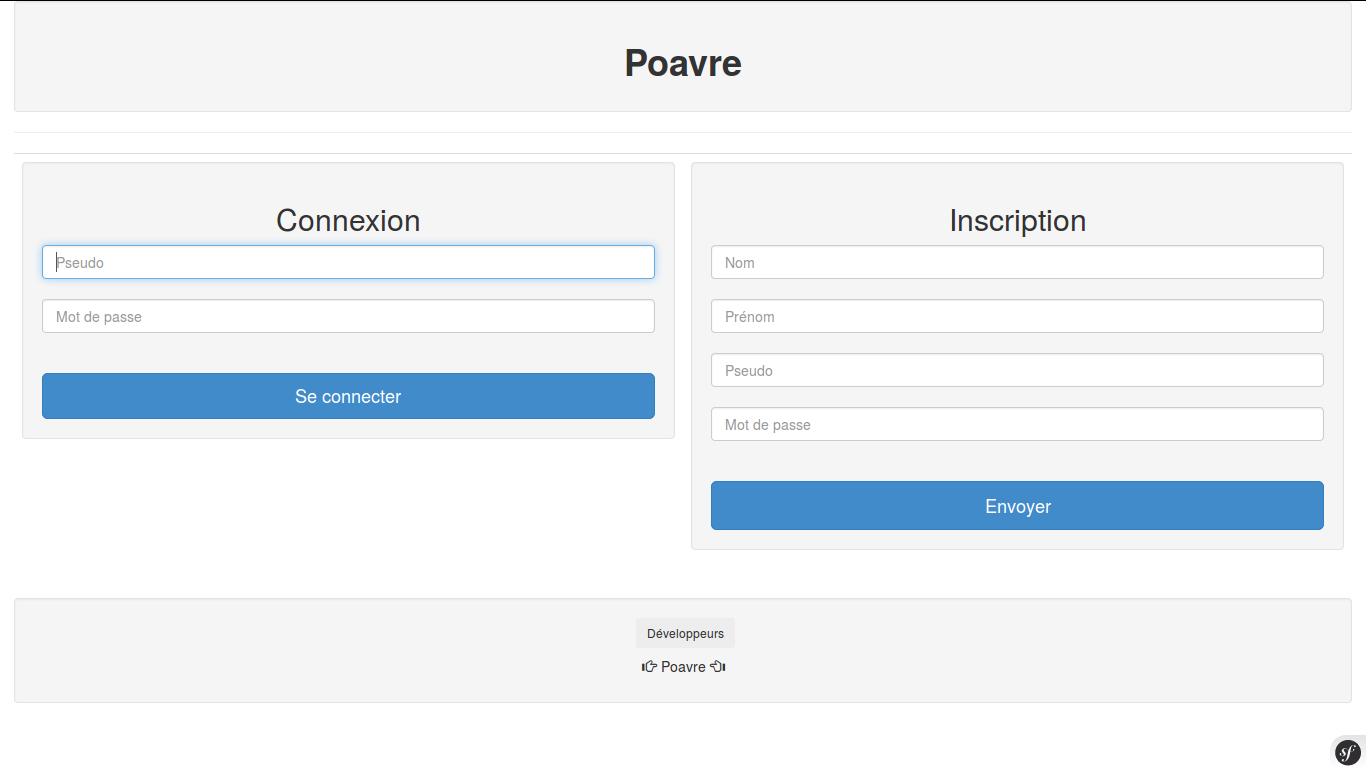
\includegraphics[width=0.9\textwidth]{inscription}
\caption{Capture d'écran d'une inscription/connexion}
\label{fig:Inscription}
\end{figure}

Lorsque le visiteur désormais nommé utilisateur est connecté (voir figure \ref{fig:Profil}) il peut à tout moment se déconnecter, éditer son profil (nom, prénom et/ou mot de passe).

\begin{figure}[h!]
\centering
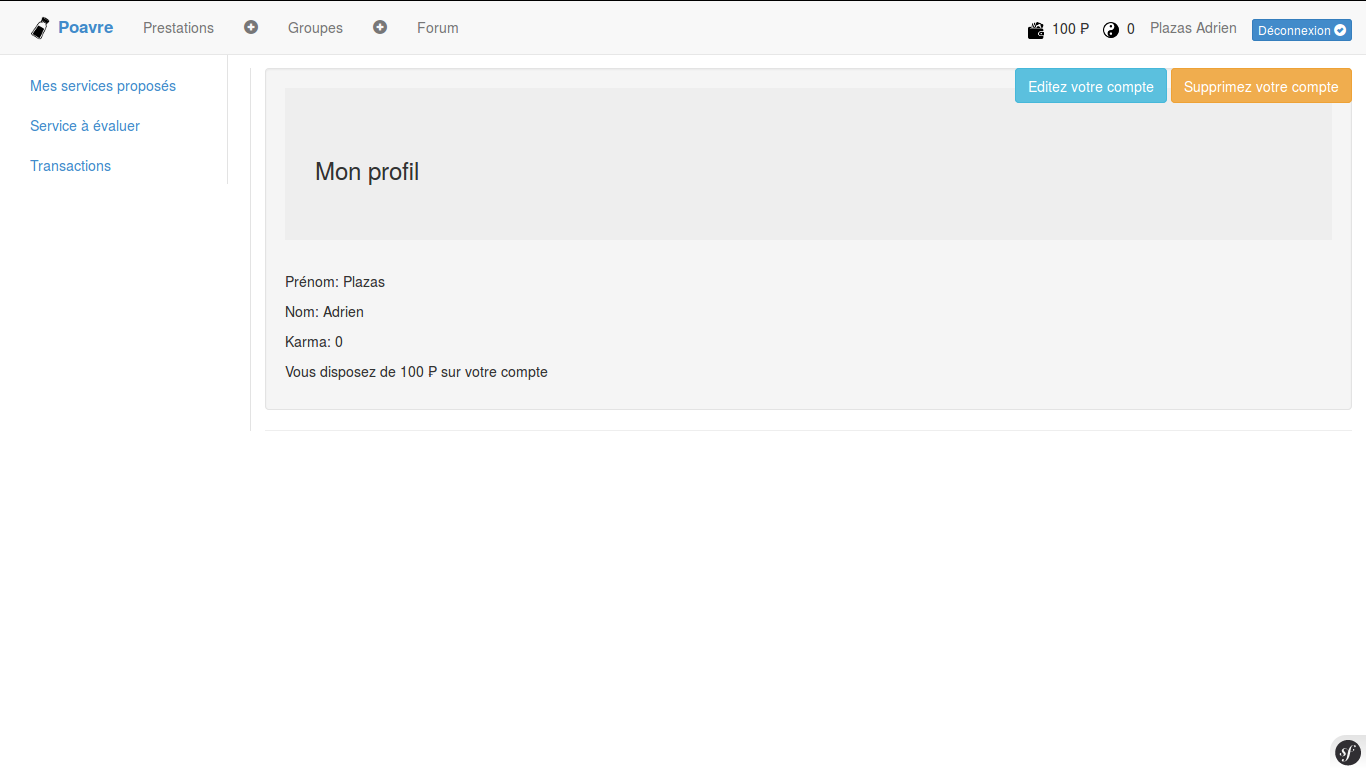
\includegraphics[width=0.9\textwidth]{profil}
\caption{Capture d'écran du profil}
\label{fig:Profil}
\end{figure}

Il peut accéder aux différents services proposés sur le site. 
Ces derniers peuvent être des services de covoiturage, de couchsurfing, de vente ou un autre type de service nommé «~service de base~».

Ainsi, il peut réserver un service, dans ce cas, le créateur du service se doit de le réaliser ce qui entraînera par la suite une obligation de transaction entre l'utilisateur et le créateur du service ainsi qu'une évaluation par la personne ayant bénéficiée du service (voir figure \ref{fig:Montre}).

\begin{figure}[h!]
\centering
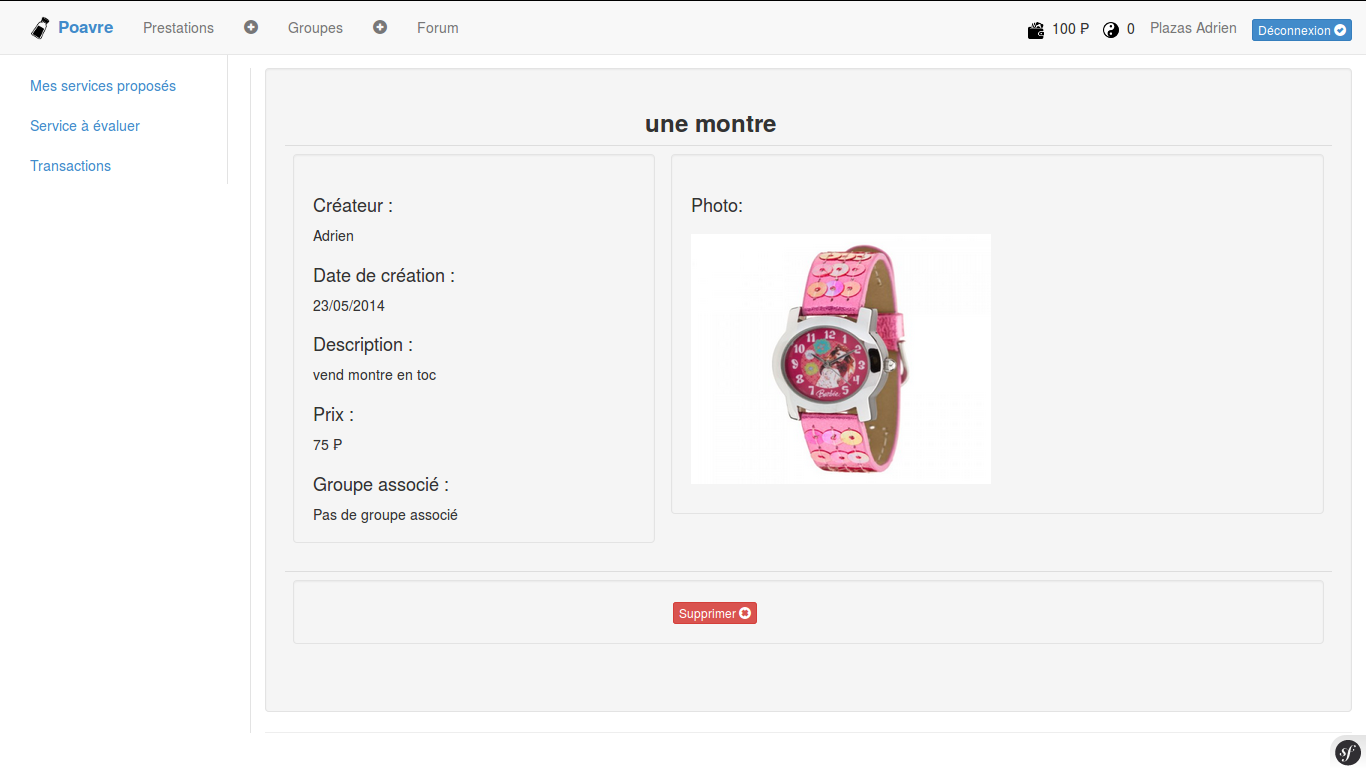
\includegraphics[width=0.9\textwidth]{montre}
\caption{Capture d'écran d'une réservation}
\label{fig:Montre}
\end{figure}

Chaque utilisateur peut également créer son propre service, il peut à tout moment l'annuler, il disparaît ainsi de la liste des services proposés sur le site (voir figure \ref{fig:Vente}).

\begin{figure}[h!]
\centering
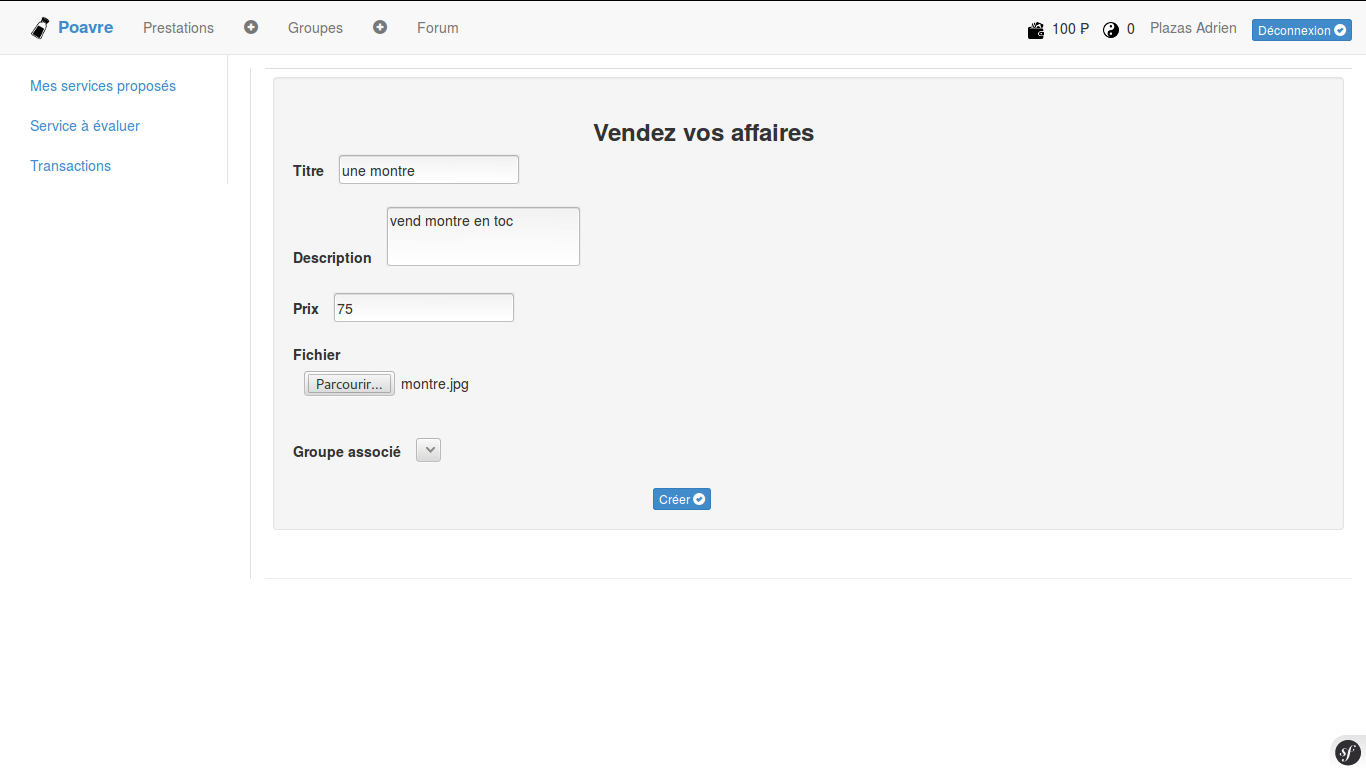
\includegraphics[width=0.9\textwidth]{vente}
\caption{Capture d'écran d'une vente}
\label{fig:Vente}
\end{figure}

L'utilisateur ne peut quitter le site que s'il a clôturé tous les services qu'il a réservé (un mail de contact est cependant disponible pour une suppression complète).
Par ailleurs, un utilisateur peut voir la liste des groupes présents sur le site, il peut candidater pour rejoindre ces différents groupes et peut à tout moment annuler sa demande. Il peut aussi visualiser pour chaque groupe la liste de ses membres ainsi que les services qui lui sont associés.
Lorsque l'utilisateur fait parti d'un groupe il peut quitter ce dernier s'il le souhaite.
Un utilisateur peut aussi créer son propre groupe en ajoutant des utilisateurs à ce dernier. Seuls un nom de groupe et une description sont demandés pour la création d'un groupe.
Un administrateur de groupe peut bannir les membres du groupe ou en ajouter de nouveaux et il peut voir la liste des candidatures pour rejoindre le groupe et les accepter ou refuser.
Il peut à tout moment dissoudre le groupe, dans ce cas, tous les services associés au groupe ne le sont plus, ils ne disparaissent cependant pas du site (voir figure \ref{fig:Groupe}).

\begin{figure}[h!]
\centering
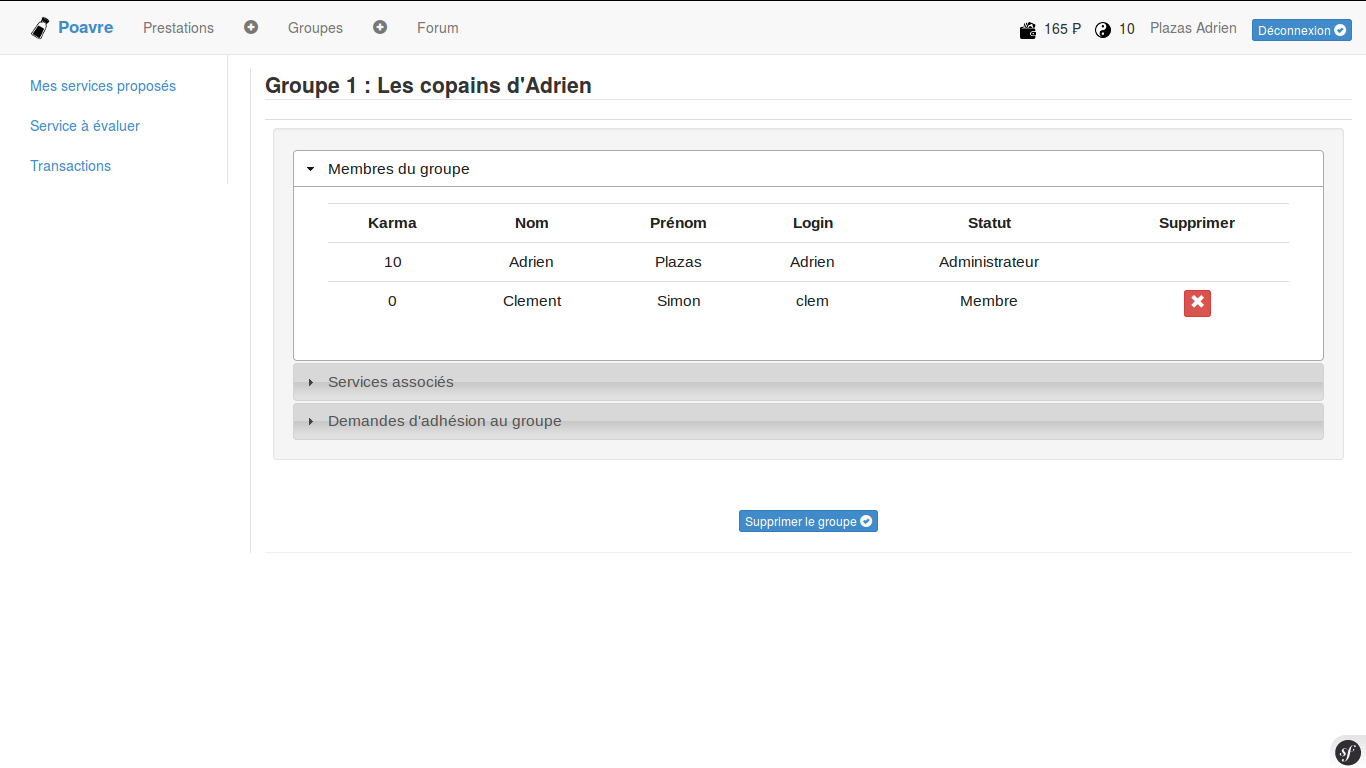
\includegraphics[width=0.9\textwidth]{groupe}
\caption{Capture d'écran d'un groupe}
\label{fig:Groupe}
\end{figure}

Un membre du site peut accéder aux différents services qu'il propose ainsi qu'aux services qu'on lui a réservé. Par ce dernier cas, il peut confirmer qu'un service a bien été effectué et après cela il peut évaluer le membre qui a réalisé le service. 
Cette évaluation permet à ce dernier d'obtenir des points de karma et déclenche la transaction entre les deux utilisateurs (voir figure \ref{fig:Evaluation}).

\begin{figure}[h!]
\centering
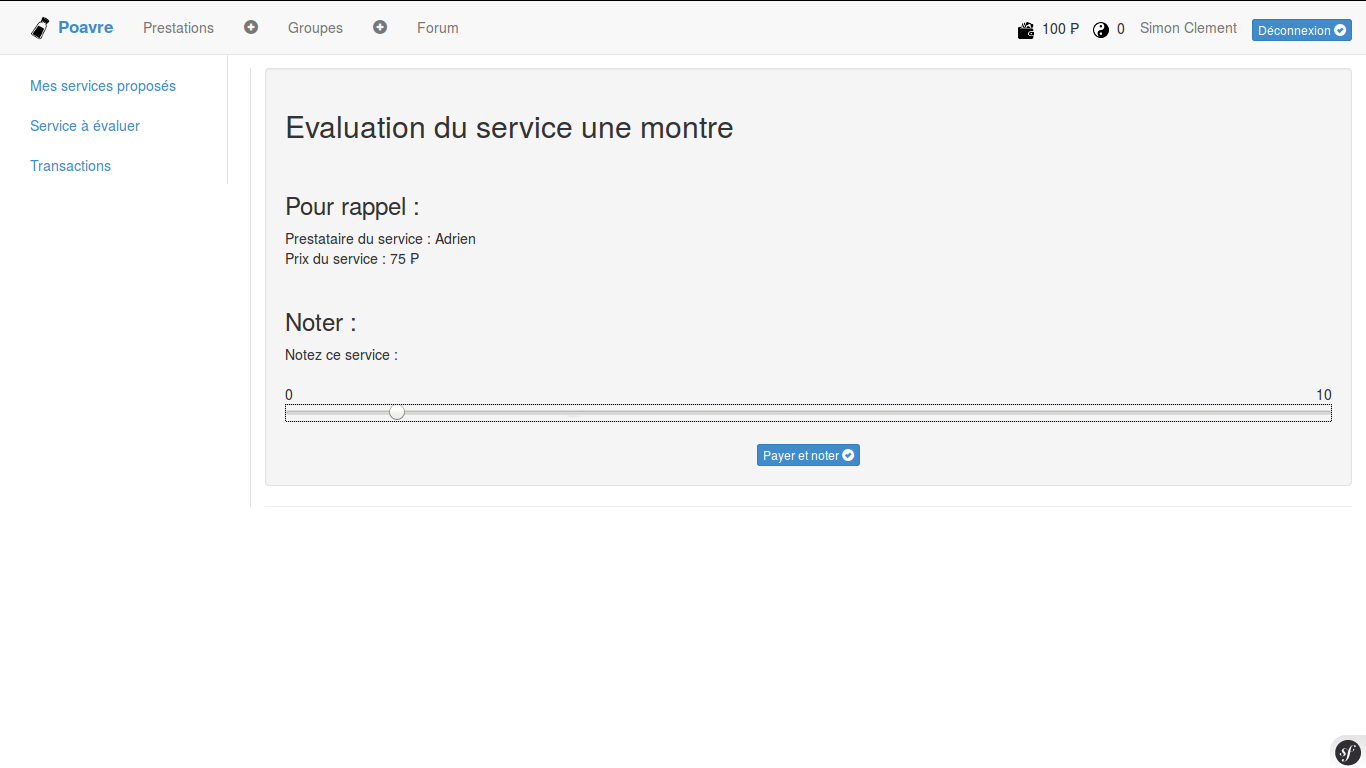
\includegraphics[width=0.9\textwidth]{achat}
\caption{Capture d'écran d'une évaluation}
\label{fig:Evaluation}
\end{figure}

A tout moment l'utilisateur peut visualiser le nombre de points de karma dont il dispose ainsi que l'argent qu'il possède.
Un utilisateur ne peut réserver un service que s'il dispose des fonds nécessaires pour payer le service (l'argent qu'il doit à un autre utilisateur est pris en compte dans ce calcul).
L'utilisateur peut visualiser la liste de ses transactions avec les autres utilisateurs et peut réaliser des paiements qualifiés de «~dons~» avec les autres utilisateurs (voir figure \ref{fig:Transaction}).

\begin{figure}[h!]
\centering
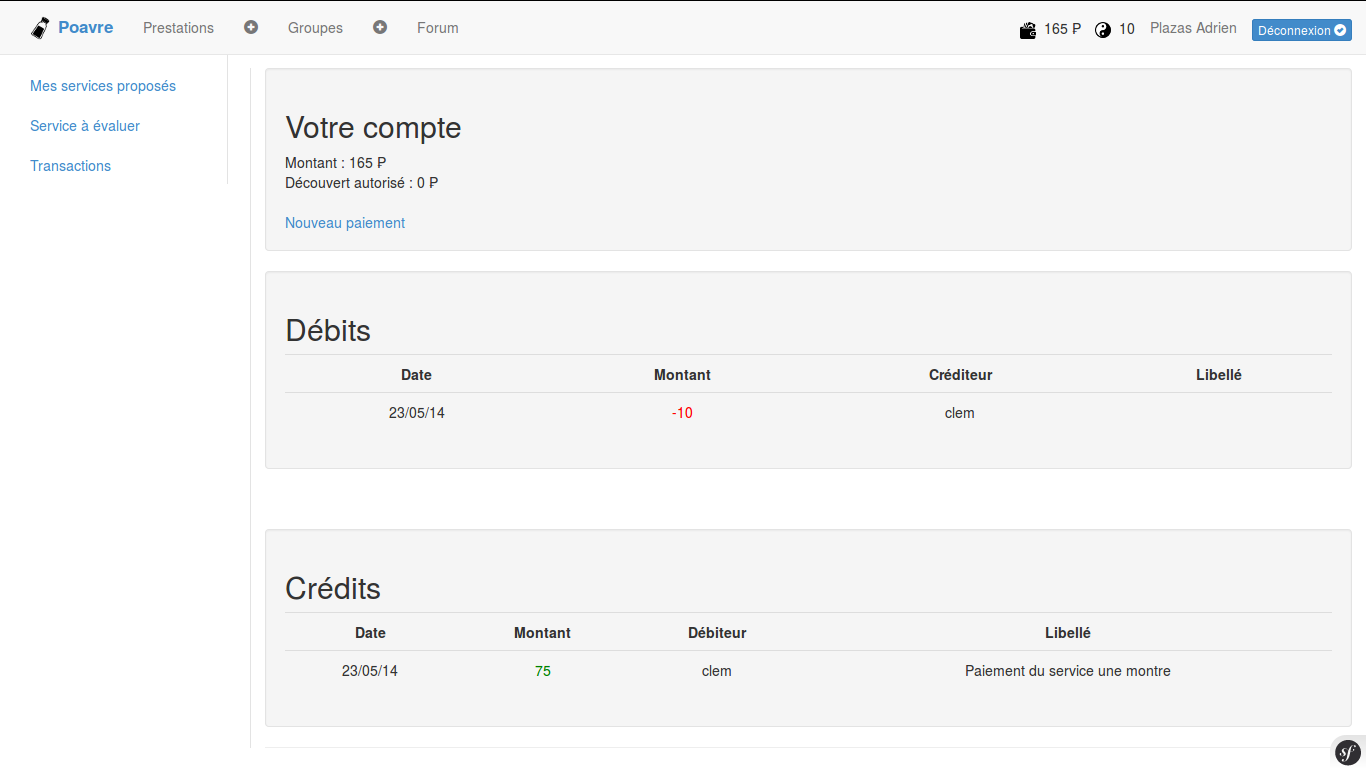
\includegraphics[width=0.9\textwidth]{trans}
\caption{Capture d'écran d'une transaction}
\label{fig:Transaction}
\end{figure}

Un membre du site peut accéder au Forum, par celui-ci il peut visualiser la liste des différents «~topics~» (ou «~sujets~») classés par ratios («~likes~»/«~dislikes~») décroissants (voir figure \ref{fig:Liste_Forum}).

\begin{figure}[h!]
\centering
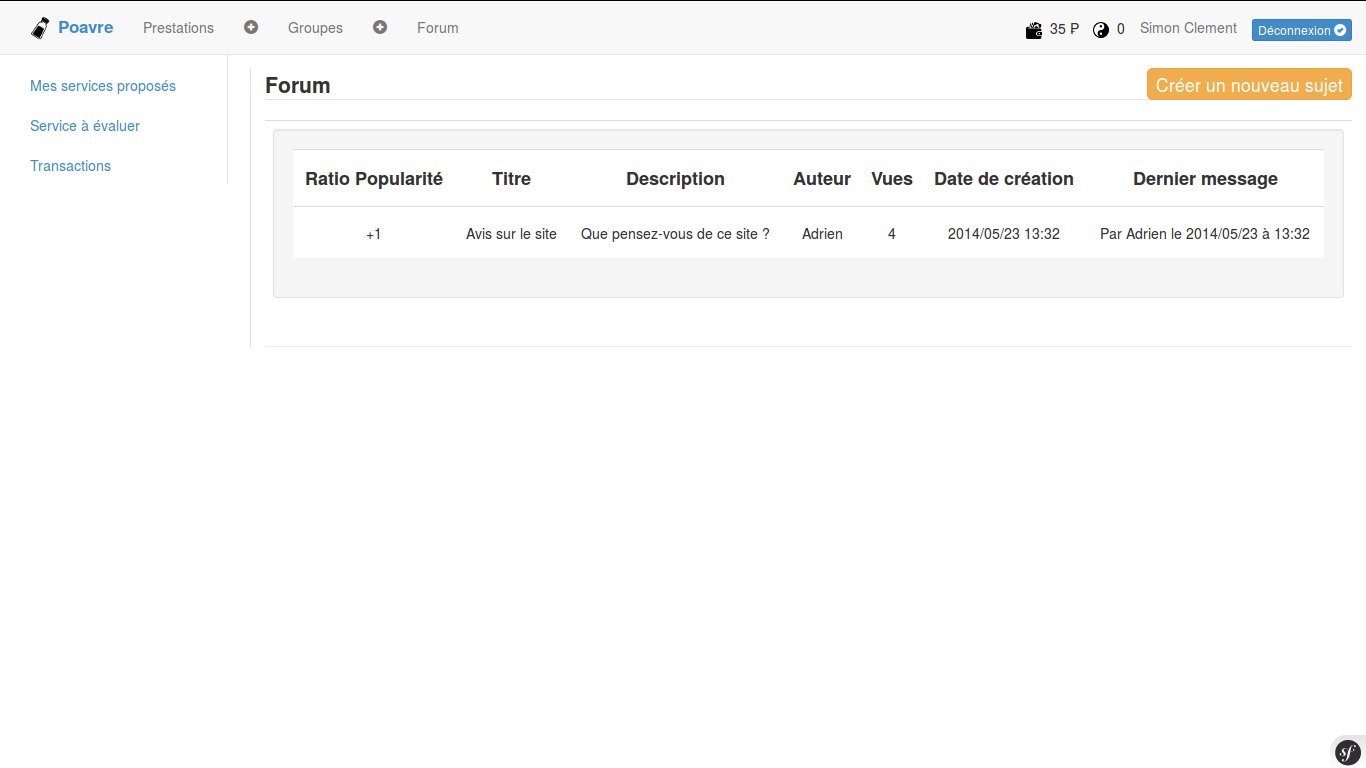
\includegraphics[width=0.9\textwidth]{liste_forum}
\caption{Capture d'écran de la liste des topics}
\label{fig:Liste_Forum}
\end{figure}

Il peut ainsi accéder à un topic, commenter celui-ci ou encore l'évaluer par un «~like~» ou un «~dislike~». 
Bien évidemment l'utilisateur peut lui-même créer un topic (voir figure \ref{fig:Forum}).

\begin{figure}[h!]
\centering
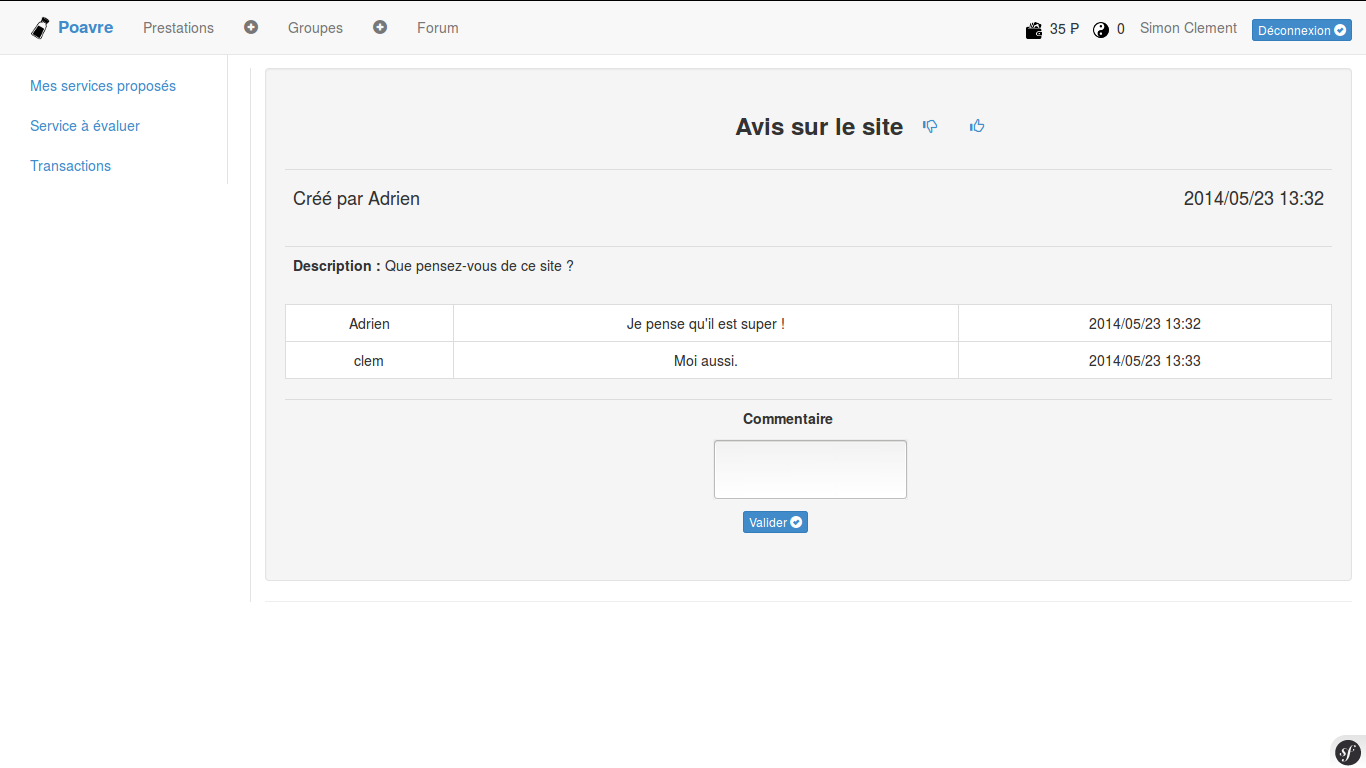
\includegraphics[width=0.9\textwidth]{forum}
\caption{Capture d'écran du forum}
\label{fig:Forum}
\end{figure}

De plus, un utilisateur bénéficiant des droits d'administration peut accéder à l'espace d'administration du site.
Depuis ce dernier, il peut bannir des utilisateurs, leur accorder les droits d'administration ou les droits «~suprêmes~», il peut aussi supprimer des services qu'il juge non-conformes, des groupes, des topics ou encore des commentaires sur les topics. Les droits «~suprêmes~» fournissent à un utilisateur un rôle de dirigeant du site. Les dirigeants ne peuvent pas se bannir entre eux.



\chapter{Bilan de ce projet}
% auteur : Fabien, Florian
% relu par : Clément, Florian, Fabien

Le travail collaboratif nécessite beaucoup d'organisation, notamment lorsqu'il s'agit d'un travail de groupe à 8. En effet, la coordination entre les membres s'est avérée difficile, bien que chacun ait travaillé sur des parties indépendantes.
Des outils simples et efficaces se sont révélés indispensables, de ce fait, Producteev et Github ont été d'une grande utilité et Symfony2 fut un très bon choix du fait de ses performances. Cela a cependant également été source de ralentissement en début de semestre, certains membres du groupe devant apprendre le fonctionnement de git, ou le temps de comprendre le fonctionnement de Symfony2.

Les réunions de projet qu'elles aient été formelles ou informelles ont apportées beaucoup au projet, elles en ont été le fondement. Elles ont permis à de nombreuses reprises de discuter et d'évacuer les tensions qui avaient pu apparaître entre les membres du groupe.
De façon globale, nous avons appréciés travailler ensemble, malgré les difficultés. En effet, nous avons avec satisfaction produit un site fonctionnel, en trouvant au fur et à mesure de l'avancée du semestre une certaine synergie qui nous a permis de travailler de façon agréable et efficace.



\chapter{Perspectives et conclusions}
% auteur : Fabien
% relu par : Clément Florian Oualid

Des perspectives de développement demeurent, à savoir~:
\begin{itemize}
    \item un système de chat privé (discussion instantanée et/ou message avec sujet) entre les utilisateurs afin de discuter des services qu'ils proposent~;
    \item l'implémentation du compte premium imaginé n'a pas été utilisé finalement dans le projet (système de gain en monnaie libre contre des euros, par exemple)~;
    \item la mise en place d'avatars qui pourront être utiles notamment pour le forum et le chat privé.
\end{itemize}

Les kiwis (mini-avatars représentatifs de l'échelon social de l'utilisateur sous forme de poivriers ou de grains de poivre par exemple), initialement prévus n'ont pas vus le jour et sont donc implémentables dans un futur proche. Aussi, une barre latérale présentant les services qui sont proposés par les utilisateurs possédant des hauts karmas pourrait être implémentée sur les vues liées aux services.

Finalement, la majeure partie des idées énoncées lors des premières réunions de projet ont été réalisées, le diagramme des cas d'utilisation ainsi que le diagramme de classe initiaux ont globalement été bien suivis.
En effet, un utilisateur peut créer des services en échange de la monnaie libre choisie, il peut gérer ses services et en réserver d'autres.
Il peut aussi évaluer un service réalisé par un prestataire ce qui donne des points de karma au prestataire, de ce fait, il gagne en «~confiance~» et ses services en sont valorisés et deviennent attrayants.
Un utilisateur peut aussi créer un groupe, rejoindre un groupe et créer des services associés à un groupe, ainsi, les services internes au groupe sont accessibles plus facilement par les membres du groupes et peuvent être catégorisés selon le désir du fondateur du groupe.
Aussi, plusieurs types de services sont disponibles, à savoir, les ventes, le couchsurfing, le covoiturage ainsi que d'autres services que nous considérons comme des services de base (cours d'anglais par exemple).
Un forum est également disponible afin de communiquer entre membres de Poavre, le forum fonctionne par topics et par commentaires de topics. Les topics sont classés par ratio (likes/dislikes) afin de faire remonter les plus intéressants.
Un espace administrateur est disponible afin de gérer le site et ses diverses fonctionnalités.


%Chapitres annexes, notés avec des lettres capitales

\appendix

\chapter{Code}

\section{Exemple de modèle}

\subsection{src/Ml/TransactionBundle/Entity/Transaction.php}
\lstinputlisting{../Symfony/src/Ml/TransactionBundle/Entity/Transaction.php}
\subsection{src/Ml/TransactionBundle/Entity/Account.php}
\lstinputlisting{../Symfony/src/Ml/TransactionBundle/Entity/Account.php}
\subsection{src/Ml/TransactionBundle/Entity/Evaluation.php}
\lstinputlisting{../Symfony/src/Ml/TransactionBundle/Entity/Evaluation.php}
\subsection{src/Ml/TransactionBundle/Entity/BasicEval.php}
\lstinputlisting{../Symfony/src/Ml/TransactionBundle/Entity/BasicEval.php}

\section{Exemple de formulaire}

\subsection{src/Ml/UserBundle/Form/UserType.php}
\lstinputlisting{../Symfony/src/Ml/UserBundle/Form/UserType.php}

\section{Exemple d'exception}

\subsection{src/Ml/TransactionBundle/Exception/TransactionException.php}
\lstinputlisting{../Symfony/src/Ml/TransactionBundle/Exception/TransactionException.php}
\subsection{src/Ml/TransactionBundle/Exception/RefusedTransactionException.php}
\lstinputlisting{../Symfony/src/Ml/TransactionBundle/Exception/RefusedTransactionException.php}

\section{Exemple de contôleur}

\subsection{src/Ml/TransactionBundle/Controller/TransactionController.php}
\lstinputlisting{../Symfony/src/Ml/TransactionBundle/Controller/TransactionController.php}

\section{Exemple de routes}
\subsection{src/Ml/TransactionBundle/Resources/config/routing.yml}
\lstinputlisting{../Symfony/src/Ml/TransactionBundle/Resources/config/routing.yml}

\section{Exemple de vues}

\subsection{app/Resources/views/layout.html.twig}
\lstinputlisting{../Symfony/app/Resources/views/layout.html.twig}
\subsection{app/Resources/views/headerbar.html.twig}
\lstinputlisting{../Symfony/app/Resources/views/headerbar.html.twig}
\subsection{src/Ml/TransactionBundle/Resources/views/Transaction/index.html.twig}
\lstinputlisting{../Symfony/src/Ml/TransactionBundle/Resources/views/Transaction/index.html.twig}
\subsection{src/Ml/UserBundle/Resources/views/User/edit.html.twig}
\lstinputlisting{../Symfony/src/Ml/UserBundle/Resources/views/User/edit.html.twig}



\chapter{Documentation des espaces de nommage}
\import{latex/}{namespaceMl}
\import{latex/}{namespaceMl_1_1AdministrationBundle}
\import{latex/}{namespaceMl_1_1AdministrationBundle_1_1Controller}
\import{latex/}{namespaceMl_1_1ForumBundle}
\import{latex/}{namespaceMl_1_1ForumBundle_1_1Controller}
\import{latex/}{namespaceMl_1_1ForumBundle_1_1Form}
\import{latex/}{namespaceMl_1_1GroupBundle}
\import{latex/}{namespaceMl_1_1GroupBundle_1_1Controller}
\import{latex/}{namespaceMl_1_1HomeBundle}
\import{latex/}{namespaceMl_1_1HomeBundle_1_1Controller}
\import{latex/}{namespaceMl_1_1libServices}
\import{latex/}{namespaceMl_1_1ServiceBundle}
\import{latex/}{namespaceMl_1_1ServiceBundle_1_1Controller}
\import{latex/}{namespaceMl_1_1ServiceBundle_1_1Form}
\import{latex/}{namespaceMl_1_1TransactionBundle}
\import{latex/}{namespaceMl_1_1TransactionBundle_1_1Controller}
\import{latex/}{namespaceMl_1_1TransactionBundle_1_1Exception}
\import{latex/}{namespaceMl_1_1UserBundle}
\import{latex/}{namespaceMl_1_1UserBundle_1_1Controller}
\import{latex/}{namespaceMl_1_1UserBundle_1_1Form}
\chapter{Documentation des classes}
\import{latex/}{classMl_1_1AdministrationBundle_1_1Controller_1_1AdministrationController}
\import{latex/}{classMl_1_1ServiceBundle_1_1Form_1_1BasicType}
\import{latex/}{classMl_1_1ServiceBundle_1_1Form_1_1CarpoolingType}
\import{latex/}{classMl_1_1ForumBundle_1_1Form_1_1CommentType}
\import{latex/}{classMl_1_1ServiceBundle_1_1Form_1_1CouchSurfingType}
\import{latex/}{classMl_1_1TransactionBundle_1_1Controller_1_1EvaluationController}
\import{latex/}{classMl_1_1ForumBundle_1_1Controller_1_1ForumController}
\import{latex/}{classMl_1_1GroupBundle_1_1Controller_1_1GroupController}
\import{latex/}{classMl_1_1HomeBundle_1_1Controller_1_1HomeController}
\import{latex/}{classMl_1_1AdministrationBundle_1_1MlAdministrationBundle}
\import{latex/}{classMl_1_1ForumBundle_1_1MlForumBundle}
\import{latex/}{classMl_1_1GroupBundle_1_1MlGroupBundle}
\import{latex/}{classMl_1_1HomeBundle_1_1MlHomeBundle}
\import{latex/}{classMl_1_1ServiceBundle_1_1MlServiceBundle}
\import{latex/}{classMl_1_1TransactionBundle_1_1MlTransactionBundle}
\import{latex/}{classMl_1_1UserBundle_1_1MlUserBundle}
\import{latex/}{classMl_1_1TransactionBundle_1_1Exception_1_1RefusedTransactionException}
\import{latex/}{classMl_1_1libServices_1_1ReservationTested}
\import{latex/}{classMl_1_1ServiceBundle_1_1Form_1_1SaleType}
\import{latex/}{classMl_1_1ServiceBundle_1_1Controller_1_1ServiceController}
\import{latex/}{classMl_1_1libServices_1_1SessionTested}
\import{latex/}{classMl_1_1ForumBundle_1_1Form_1_1TopicType}
\import{latex/}{classMl_1_1TransactionBundle_1_1Controller_1_1TransactionController}
\import{latex/}{classMl_1_1TransactionBundle_1_1Exception_1_1TransactionException}
\import{latex/}{interfaceMl_1_1TransactionBundle_1_1Exception_1_1TransactionExceptionInterface}
\import{latex/}{classMl_1_1UserBundle_1_1Controller_1_1UserController}
\import{latex/}{classMl_1_1UserBundle_1_1Form_1_1UserType}
\chapter{Documentation des fichiers}
\import{latex/}{AdministrationController_8php}
\import{latex/}{MlAdministrationBundle_8php}
\import{latex/}{ForumController_8php}
\import{latex/}{CommentType_8php}
\import{latex/}{TopicType_8php}
\import{latex/}{MlForumBundle_8php}
\import{latex/}{GroupController_8php}
\import{latex/}{MlGroupBundle_8php}
\import{latex/}{HomeController_8php}
\import{latex/}{MlHomeBundle_8php}
\import{latex/}{ReservationTested_8php}
\import{latex/}{SessionTested_8php}
\import{latex/}{ServiceController_8php}
\import{latex/}{BasicType_8php}
\import{latex/}{CarpoolingType_8php}
\import{latex/}{CouchSurfingType_8php}
\import{latex/}{SaleType_8php}
\import{latex/}{MlServiceBundle_8php}
\import{latex/}{EvaluationController_8php}
\import{latex/}{TransactionController_8php}
\import{latex/}{RefusedTransactionException_8php}
\import{latex/}{TransactionException_8php}
\import{latex/}{MlTransactionBundle_8php}
\import{latex/}{UserController_8php}
\import{latex/}{UserType_8php}
\import{latex/}{MlUserBundle_8php}


